\documentclass{article}

\usepackage[utf8x]{inputenc}
\usepackage[italian]{babel}
\usepackage{listings}
\usepackage{fullpage}
\usepackage{xcolor}
\usepackage{hyperref}
\usepackage{marvosym}
\usepackage{graphicx}


\newcommand{\knizPar}[3]{%
  \parbox[t]{0.15\textwidth}{\footnotesize
  \textbf{#1\\#2}}&\parbox[t]{0.85\textwidth}{%
    %\textbf{#3}%
    \hspace{1.5em}#3
    \vspace{\parsep}%
  }\\\\}

\title{\textbf{ Device files /dev/random e /dev/urandom}\\[0.2cm]Analisi di
algoritmi e implementazione}
\author{Emanuele Paracone \\ \texttt{emanuele.paracone@gmail.com}}


\begin{document}
\maketitle
 
%\include{sections/section0}

\section*{\centering{Il nostro lavoro e LRNG}}
\paragraph{}In questo lavoro presentiamo l'analisi degli algoritmi e
dell'implementazione dei device file \textbf{/dev/random} e
\textbf{/dev/urandom}.
Tale elaborato è previsto a conclusione del corso di
\emph{\textbf{Linux Avanzato}} per l'\emph{A. A. 2013-2014} 

\paragraph{} Il nostro obiettivo è fornire un'analisi del \emph{Linux
Random Number Generator} (\emph{LRNG}), il generatore di numeri pseudocasuali del
kernel Linux, attraverso una descrizione delle sue struttura e
implementazione. Nello specifico, abbiamo analizzato la versione del kernel
3.14.4.

\section*{Una panoramica su LRNG\ldots}
 
\paragraph{}L'implementazione del \emph{PseudoRandomNumberGenerator} (PRNG) di
Linux risiede sostanzialmente nelle $\sim~$1700 righe di codice del file sorgente
\verb$drivers/char/random.c$, scritto da Matt Mackall e Theodore Ts'o (\cite{mack}).
\paragraph{} Il LRNG è oggetto di particolare interesse per il ruolo che ricopre
in applicazioni relative alla sicurezza per le quali è cruciale l'uso di un
generatore di numeri pseudocasuali di buona qualità. 
\paragraph{}A dispetto di quanto ci si
aspetterebbe, sebbene il LRNG sia stato inserito nel kernel nel 1994, non
abbiamo trovato sue documentazioni o descrizioni in letteratura antecedenti
l'articolo di Zvi Gutterman, Benny Pinkas, and Tzachy Reinman \emph{Analysis of the Linux
random number generator} \cite{gutt}, pubblicato nel 2006 e con oggetto la
versione del kernel 2.6.10. In questo lavoro faremo spesso riferimento all'articolo di
Gutterman e, soprattutto, al più recente \emph{The linux pseudorandom number
generator revisited} di Patrick Lacharme, Andrea Röck, Vincent Strubel, and
Marion Videau \cite{lach}  pubblicato nel 2012, che effettua una nuova analisi
su un kernel più recente (2.6.30.7) e suggerisce alcune modifiche
dell'implementazione che sono state accolte nelle versioni attuali del kernel.

\subsection*{LRNG nel kernel 3.14.4}

\paragraph{}La nostra analisi si concentrerà sulle caratteristiche funzionali
del LRNG e sulla sua implementazione. Nelle sezioni che seguono diamo una
descrizione delle sue:
\begin{enumerate} 
  \item struttura;
  \item gestione degli input di entropia esterna;
  \item produzone degli output;
  \item implementazione dei requisiti di sicurezza; 
  \item storia ed evoluzione recente.
\end{enumerate}
A corredo del lavoro presente esponiamo il codice sorgente di \verb+random.c+ su
\textbf{github} \cite{kniz} con i nostri commenti al codice (che si distinguono
da quelli originali perché riportati in lingua italiana).

\section{La Struttura del LRNG}
  
 \subsection{Un po' di notazione}\label{notazione}
 \knizPar{}{Gli \emph{Entropy \\Inputs}}{Il PRNG di Linux
 rientra nella classificazione di \emph{Pseudorandom Number Generator} con \emph{entropy inputs}, ovvero è un
 generatore di numeri pseudocasuali i cui bit di output sono prodotti in modo
 non deterministico per l'introduzione di input da sorgenti esterne di entropia
 (\textbf{entropy inputs}). Detti input aggiornano il generatore introducendo
 impredicibilità nei possibili valori che può assumerne lo \textbf{stato
 interno}.}
  \centerline{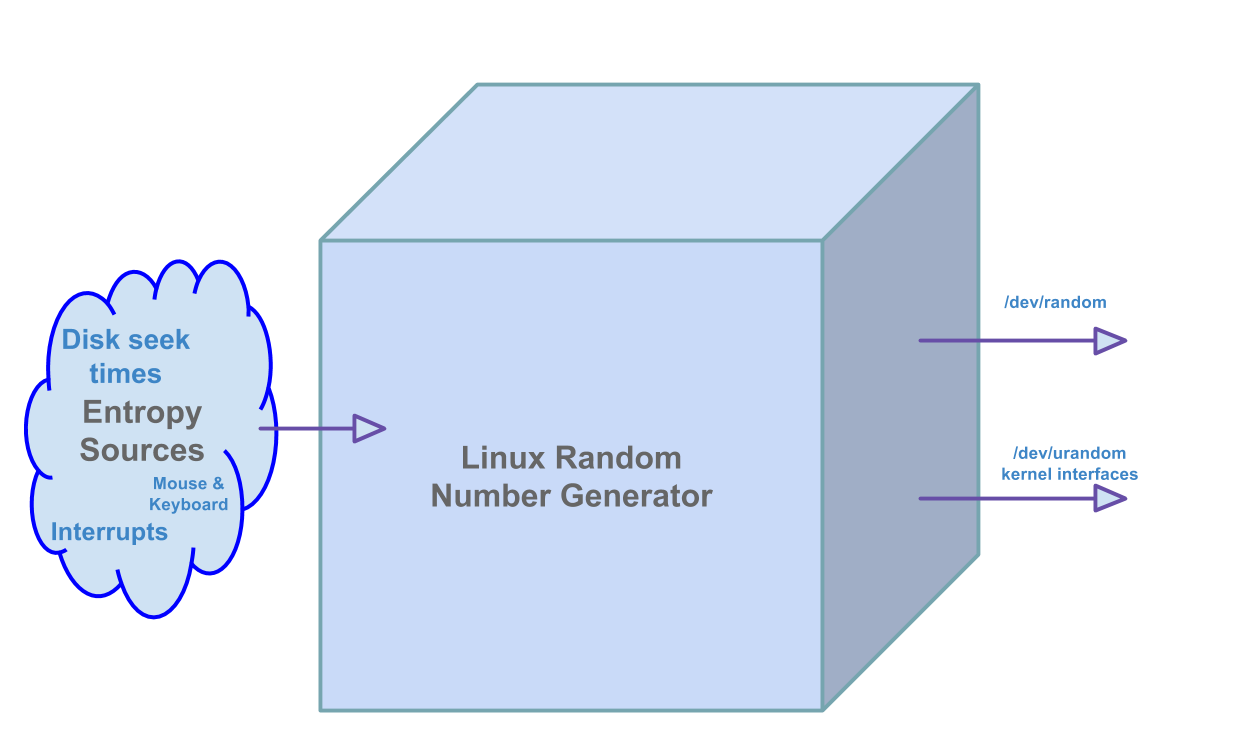
\includegraphics[width=150mm]{img/entropy_sources.png}}
 
 \knizPar{L'Entropia}{}{Poiché si richiede che i numeri generati abbiano una
 buona ``qualità'', l'impredicibilità introdotta dagli entropy input deve poter essere
 misurata per garantire un buon livello di randomicità dei bit di output. D'ora
 in avanti utilizzeremo il termine \textbf{entropia} per indicare la
 metrica che misura il livello di randomicità che viene ``aggiunto'' allo stato interno
 del generatore a seguito di un input di entropia. }
 \knizPar{I tipi di}{\emph{Entropy Inputs}}{ Gli entropy inputs possono essere
 di tre tipi:
 \begin{itemize}
   \item \textbf{user input}: input provenienti da mouse e tastiera;
   \item \textbf{disk I/O};
   \item \textbf{interrupts}.
 \end{itemize}
 \paragraph{}L'entropia di un'entropy input è costituita dal valore dello
 specifico input e dal tempo intercorso tra l'input presente e l'ultimo input
 dello stesso tipo, misurato sia in jiffies che in cicli di CPU. 
 
 \paragraph{}Gli \emph{entropy inputs} hanno in comune la
 caratteristica di essere:
 \begin{itemize}
   \item non deterministici;
   \item difficili da misurare per un osservatore esterno
 \end{itemize}
e aggiungono entropia al generatore in modo asincrono e
 indipendente rispetto alla generazione degli output. 
 }
 
 \subsection{Struttura Generale}
 Il cuore del LRNG è un buffer protetto, cui da ora in avanti ci riferiremo col
 nome di \textbf{stato interno}, inaccessibile per via diretta. Il LRNG produce
 i propri output a partire dai valori contenuti nel suo stato interno.
 Conseguentemente, lo stato interno deve essere aggiornato non solo attraverso
 la raccolta di quanti più \emph{entropy input} possibile, ma anche ogni volta
 che viene richiesto un buffer in output al LRNG (mediante un
 opportuno meccanismo di feedback).
 
  \centerline{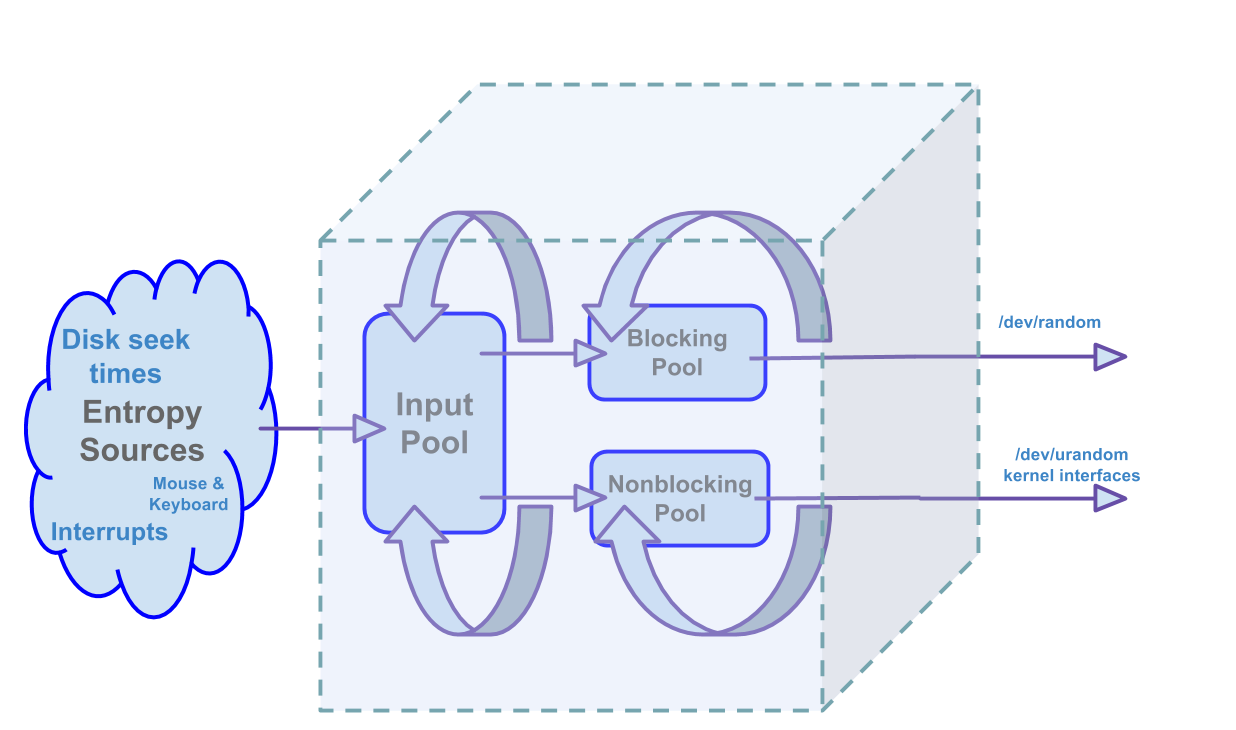
\includegraphics[width=150mm]{img/internal_state.png}}
 
 
 La sicurezza del generatore, ovvero l'impossibilità di prevedere gli output
 futuri (\emph{backward security}) una volta che siano noti gli \emph{entropy
 input} e l'impossibilità di ricostruire gli output passati (\emph{forward
 security}) a partire dalla conoscenza dello stato interno, è descritta nella
 sezione \ref{sicurezza} riguardante la sicurezza del LRNG.
 \paragraph{}In quel che segue della presente sezione diamo una breve
 descrizione dello stato interno del generatore e delle sue interfacce.
 
 \subsubsection{Lo Stato Interno e le pool}
 Lo stato interno del LRNG è rappresentato, all'interno del kernel, da tre
 strutture dette \textbf{pool}, cui nel codice viene fatto riferimento come:
 \begin{itemize}
   \item \textbf{input pool} 
   \item \textbf{blocking pool}
   \item \textbf{nonblocking pool}
 \end{itemize}
 
 \paragraph{}L'entropia aggiunta al generatore dagli \emph{entropy inputs}
 viene accumulata nella \emph{input pool} (chiamata anche \emph{pool} primaria
 in \cite{gutt}). L'entropia viene poi trasferita verso una delle altre due
 pool, \emph{blocking} o \emph{nonblocking}, generalmente (ma non solo!) in
 occasione del prelievo di bytes randomici in output dal LRNG e nella quantità
 strettamente necessaria. Per questo le pool \emph{blocking} e
 \emph{nonblocking} sono anche dette \textbf{output pool} o \emph{pool}
 secondarie (rispettivamente in \cite{lach} e \cite{gutt}). Tratteremo nel
 dettaglio la struttura delle tre pool in \ref{pool}.
 
 \subsubsection{La gestione dell'entropia}\label{aggiuntaentropia}
 \paragraph{}Il LRNG si comporta in modo diverso nel gestire
 il mantenimento dell'entropia interna a seconda che questa venga
 aggiunta o estratta rispetto alle \emph{pool}. \\
 Quando viene immessa nelle pool dell'entropia derivata dagli
 \emph{entropy input} o proveniente dalla \emph{input pool}, 
 il kernel usa una mixing function lineare per efficientare
 l'accumulazione di entropia nell'\emph{input pool} (viene preferita
 pertanto una CRC all'uso di una funzione hash sebbene la prima non sia
 crittograficamente robusta), mentre, quando viene trasferita entropia
 dalla input pool verso una output pool o vengono generati bit dalle output
 pool, il LRNG fa uso della primitiva crittografica SHA-1. \\
  È facile convincersi dei benefici introdotti da questa disparità, in quanto
 l'aggiunta di entropia rimane un'operazione veloce nonostante gli
 \emph{entropy input} abbiano un tasso di arrivo elevato (e maggiore di vari
 ordini di grandezza rispetto al tasso con cui mediamente sono richiesti gli
 output).\\ 
 Anche se ci proponiamo di definire più avanti il concetto di ``sicurezza''
 riferito al LRNG, vogliamo già dare risalto al fatto che la segretezza
 dello stato interno risieda fondamentalmente nell'adozione di SHA-1 per la
 produzione degli output.
 
   
  \centerline{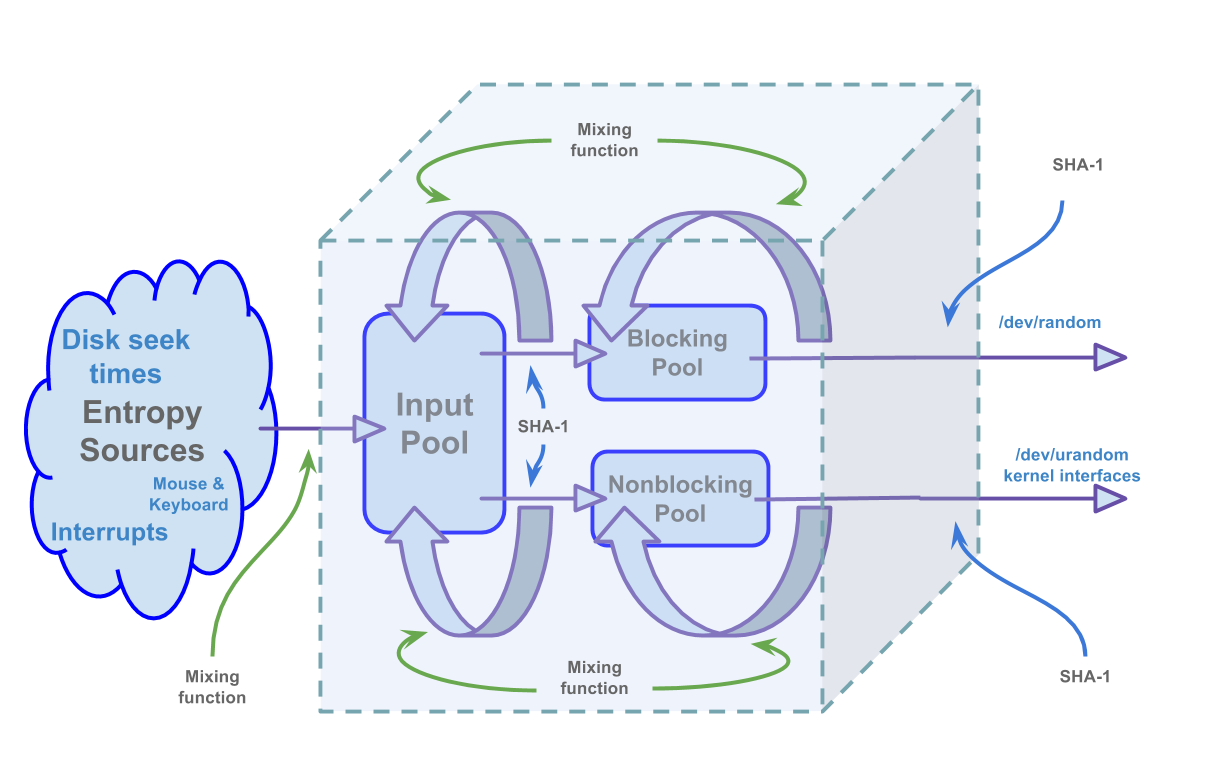
\includegraphics[width=150mm]{img/Sha1.png}}
 
 
 \paragraph{}Ogni volta che viene aggiunta dell'entropia presso una pool, viene
 aggiornato un contatore specifico per quella pool: l'\textbf{entropy counter}.
 La quantità per la quale viene incrementato il contatore è pari alla stima di
 entropia calcolata sul particolare \emph{entropy input} corrente (che come
 abbiamo già visto si basa sul valore dell'input e sul tempo di interarrivo tra
 questo e l'input dello stesso tipo che lo ha preceduto).
 \subsubsection{Le interfacce di output}\label{interfacceoutput}
 \paragraph{}Il LRNG espone due interfacce per il prelievo di
 numeri pseudo-randomici dallo spazio utente:
 \begin{itemize}
   \item il device file \verb+/dev/random+: espone verso l'user space la
   funzione di generazione di output dalla \emph{blocking pool};
   \item il device file \verb+/dev/urandom+: espone verso l'user space la
   funzione di generazione di output dalla \emph{nonblocking pool};
   
 \end{itemize}
 e alcune interfacce kernel:
 \begin{itemize}
	\item il simbolo \verb+get_random_bytes()+: l'interfaccia kernel
	principale, esporta verso il kernel space una funzione per la produzione di
	bytes generati dalla \emph{nonblocking pool};
   \item il simbolo \verb+get_random_int()+: esporta
   verso il kernel space una funzione per la produzione di bytes pseudocasuali
   crittograficamente non sicuri indipendenti dalle \emph{pool} (l'estrazione
   di valori siffatti non diminuisce l'ammontare di entropia dello stato
   intereno);
   \item il simbolo \verb+get_random_bytes_arch()+: esporta verso il kernel
   space un'interfaccia per l'uso di un eventuale hardware specifico per la 
   generazione di numeri pseudocasuali;
   \item il simbolo \verb+generate_random_uuid()+: esporta verso il kernel un
   generatore casuale di uuid che sfrutti il LRNG.
 \end{itemize}

 

\subsection{Le Pool}\label{pool}
 Poiché abbiamo visto come l'entropia del \emph{LRNG} sia collezionata per mezzo
 delle tre pool \emph{input}, \emph{blocking} e \emph{nonblocking}, non ci resta
 che analizzare quale sia il ruolo di queste e come concorrano
 nell'implementare lo stato interno.
 \subsubsection{A che servono le pool?}\label{poolACosaServono}
 Sappiamo già che la componente più profonda dello stato interno, ovvero quella
 che colleziona l'entropia proveniente dagli \emph{entropy input}, risieda
 nell'\emph{input pool}: il contenuto informativo di ogni \emph{entropy input}
 viene ``mischiato'' direttamente con il buffer in essa contenuto.
 Quando vengono richiesti bytes pseudocasuali al LRNG, questi vengono
 estratti dalla \emph{output pool} specifica per l'interfaccia invocata
 (\ref{interfacceoutput}).
 \paragraph{}I bytes prodotti a partire dalla
 \emph{blocking pool} (ovvero ottenuti da \verb+/dev/random+) hanno un'elevata
 qualità entropica (intesa in funzione di quanto la pool che li ha generati sia
 stata aggiornata con eventi non predicibili e quindi di elevato contenuto
 entropico), mentre tale qualità non è garantita per quelli prodotti dalla
 \emph{nonblocking pool} (ottenibili tamite l'uso delle altre interfacce).\\
 I primi, infatti, sono generati solo quando vi è sufficiente \emph{entropia}
 collezionata all'iterno del LRNG: se l'entropia stimata presso lo stato interno
 del generatore è inferiore al numero di bytes richiesti in output,
 il flusso prodotto da \verb+/dev/random+ si blocca fino all'``arrivo'' di nuova
 entropia in quantità sufficiente presso l'\emph{input pool}.\\ I secondi sono
 ottenuti in modo non bloccante a prescindere dalla quantità di entropia
 stimata per lo stato interno: in mancanza di entropia sufficiente dalla
 \emph{input pool}, la \emph{nonblocking pool} produce ugualmente bytes in
 output via SHA-1 a partire dal proprio stato interno. Notiamo come i bytes
 prodotti in modo non bloccante siano comunque idonei per la grande maggioranza
 delle applicazioni: un attaccante in possesso di vecchi output dovrebbe
 aver effettuato una crittoanalisi di SHA-1 che gli consenta di prevedere futuri
 output a partire da vecchi output (condizione sufficiente nel solo caso di
 esaurimento dell'entropia e assenza di \emph{entropy input}) mentre ad oggi si
 ritiene (anche se non è stato dimostrato) che una crittanalisi di questo genere
 non sia possibile.
 
 \paragraph{} Ogni volta che viene richiesto un output (o un trasferimento di
 entropia) e subito prima della consegna dell'output, viene aggiornato lo stato
 interno della pool coninvolta attraverso un meccanismo di retroazione (o
 \emph{feedback}).
 
   \centerline{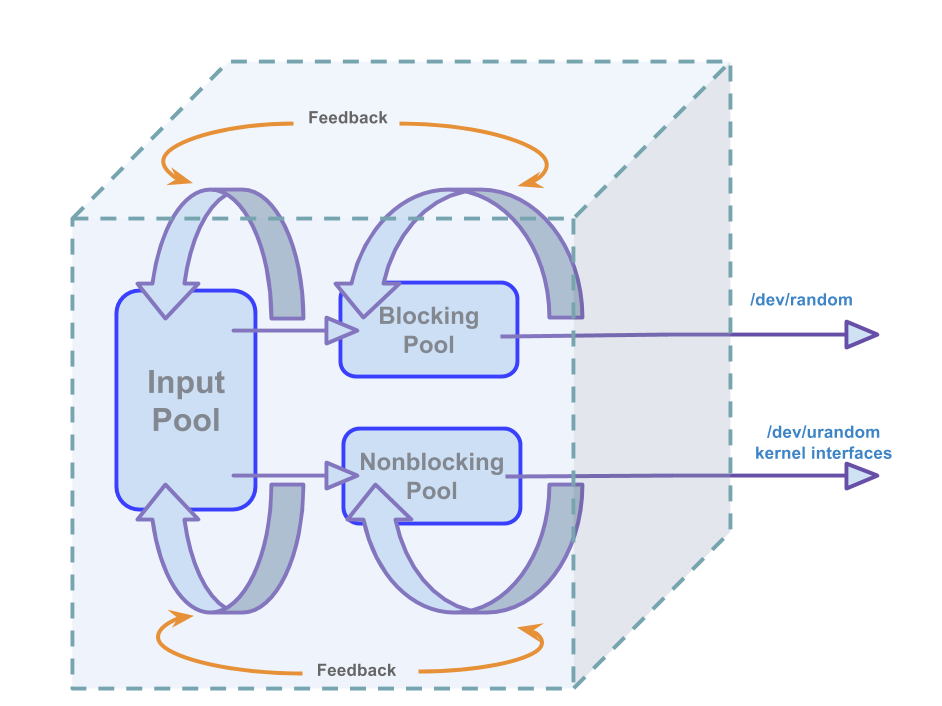
\includegraphics[width=120mm]{img/feedback.png}}
 
 
 \paragraph{}Notiamo anche che non esistano interfacce kernel per i bytes
 prodotti dalla \emph{blocking pool}: i bytes di alta qualità sono pertanto destinati
 solo per applicazioni critiche dello spazio utente. \\
 Eventuali dispositivi hardware per la generazione di numeri
 randomici sono esposti sia verso l'user space -- tramite il device driver
 \verb+hwrng+-- che verso il kernel space -- tramite il simbolo esportato 
 \verb+get_random_bytes_arch()+. Può verificarsi inoltre che un'applicazione
 nello spazio utente utilizzi gli output generati da quest'ultimo tipo di
 driver, se la sorgente è trusted, per aumentare l'affidabilità dei numeri
 generati dal \emph{LRNG}, in quanto è possibile sommare un
 seme al suo stato interno.
 \\
 La somma di un seme allo stato interno del generatore è utile all'aumento
 dell'impredicibilità dello stesso, soprattutto in fase di inizializzazione del
 sistema (quando gli entropy input sono predicibili e ridotti in numero) oppure
 nel caso di sistemi senza dischi e/o input utente. D'altro canto, l'aggiunta di
 un nuovo seme non aumenta il valore della stima dell'entropia interna delle
 varie pool.
 \subsubsection{Com'è strutturata una Pool}
 Ogni pool è modellata
 da una struttura \verb+entropy_store+ costituita sostanzialmente da:
 \begin{itemize}
   \item un buffer interno; 
   \item un \textbf{entropy counter}, che memorizza una stima dell'entropia
   aggiunta al buffer interno a partire dagli \emph{entropy inputs}
   \item un \emph{polinomio caratteristico} per la mixing function.
 \end{itemize}
 

 \paragraph{}Il buffer interno è il cuore della pool: costituisce il set di 
 registri a partire dal quale vengono effettuate le operazioni di mixing necessarie
 all'aggiunta e al perelievo di entropia. Contiene le parole (\textbf{words}) di
 16 bytes (4 unsigned a 32 bit) utilizzate dal mixing ed ha una dimensione fissata,
 specifica rispetto alla singola pool (128 \emph{words} per la \emph{input pool} e 32 per
 le \emph{output pool}). \\
 Rimandiamo il lettore alla sezione dedicata alla \emph{mixing function}
 (\ref{mixingfunction}) per una descrizione del polinomio caratteristico, e di
 come vengono prelevati e immessi bytes di entropia presso le pool.
 
 \paragraph{}I principali campi di una struttura \verb+entropy_store+ sono:\\\\
 \textbf{Campi read-only}:
 \begin{itemize}
	   \item \verb+const struct poolinfo *poolinfo+: contiene informazioni
	   sul dimensione e configurazione della pool, compreso il suo polinomio
	   caratteristico;
	   \item \verb+__u32 *pool+: punta allo stato interno della pool;
	   \item \verb+struct work_struct push_work+: punta alla funzione \verb+push_to_pool()+ 
	   (\ref{pushtopool}) nel caso in cui la pool sia un'\emph{output
	   pool}.
	 \end{itemize}
 \noindent \textbf{Campi read-write}:
 \begin{itemize}
   \item \verb+int entropy_count+: è l'\emph{entropy counter}, conta il
   numero di frazionali di bit di entropia (ottavi di 
   bit -- $2^{-3}$ bit) presenti nella pool (secondo quanto previsto dalla
   funzione di stima -- \ref{stima});
   \item \verb+unsigned short add_ptr+: contatore ciclico, indica la posizione
   della prossima parola della pool da trattare per le funzioni di mixing. 
   Le parole vengono lette in ordine inverso rispetto all'ordine nel buffer;
   \item \verb+unsigned short input_rotate+: numero di posizioni per cui devono
   essere ruotati i bit della prossima parola di entropia da aggiungere alla
   pool. Ad ogni accesso viene incrementato di 7 posizioni, ad eccezione del
   primo accesso in cui viene incrementato di 14;
   \item \verb+unsigned long last_pulled+: l'ultimo istante in jiffies in cui
   sono stati estratti bytes dalla pool;
   \item \verb+unsigned int limit+: flag di un bit impostato a 1 nel caso in
   cui la pool sia bloccante (\emph{input} e \emph{nonblocking pool}).
 \end{itemize}    
  
\subsection{I Device Files /dev/random e /dev/urandom}\label{devicefiles}
Abbiamo affermato in \ref{interfacceoutput} che vi sono due interfacce per il
prelevamento dell'output a partire dallo spazio utente costituite dai due
device files \verb+/dev/random+ e \verb+/dev/urandom+. In realtà è riduttivo
pensare a tali device file solo come interfacce per gli output del generatore: è
infatti possibile effettuare su di essi operazioni di scrittura con lo
scopo di mischiare allo stato interno un hash del valore immesso. 
\newline Le azioni specifiche per i due file sono definite nelle due
strutture \verb+file_operations random_fops+ e \\\verb+urandom_fops+.

\subsection{Dagli \emph{Entropy Input} all'Output}
Dopo aver introdotto gli ingredienti principali che costituiscono il generatore,
vediamo ora come interagiscono fra di loro.

  
 \section{L'Input}
 Gli input immessi nel LRNG possono essere solo di due tipi:
\begin{enumerate}
  \item seed aggiunto al generatore direttamente dallo spazio utente
  (\ref{poolACosaServono}).
  \item \emph{entropy input} (introdotti in \ref{notazione});
\end{enumerate}
 Nella sezione presente analizziamo l'aggiunta di entropia presso le pool
 conseguente l'arrivo di nuovi \emph{entropy input} e gli accorgimenti necessari
 per garantire la sicurezza del LRNG anche nel caso in cui l'entropia sia
 quantitativamente scarsa o nulla (per l'assenza di \emph{input}).
 
 \subsection{Il Reseeding da Spazio Utente}\label{reseeding}
 Come visto in \ref{devicefiles}, l'operazione di scrittura di un buffer
 direttamente presso i device files \verb+/dev/random+ e \verb+/dev/urandom+
 comporta un reseeding dello stato interno del generatore a partire da un hash
 del buffer stesso. 
 
    \centerline{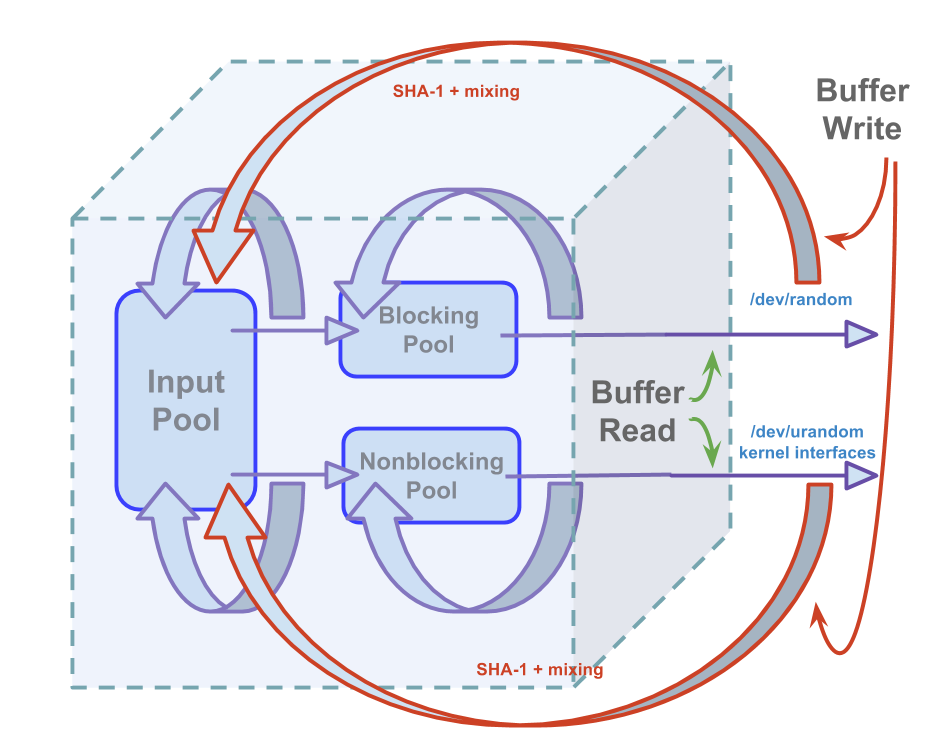
\includegraphics[width=120mm]{img/bufferRW.png}}
 
 
 Tale operazione è incoraggiata nell'header di
 \verb+random.c+, dove viene specificato che, per differenziare gli output
 prodotti in prossimità del momento del boot della macchina, è opportuna
 l'esecuzione di uno script all'avvio che scriva presso \verb+random+ o
 \verb+urandom+ un buffer letto dagli stessi device files prima dello shutdown
 della macchina. In questo modo il sistema appena avviato produrrà output
 differenti, rispetto a quelli prodotti a ridosso di altri startup dello stesso
 sistema, anche quando è stata raccolta ancora poca (o nulla) entropia
 (fatto inevitabile a ridosso dell'inizializzazione del sistema).
 Ovviamente, nel caso non siano presenti dispositivi per la memorizzazione
 persistente (dischi, flash, ecc) non è possibile adottare un simile
 accorgimento.
 \paragraph{} Vi sono altri scenari per cui può rendersi opportuno imporre
 un reseeding dello stato interno del generatore. Ad esempio, si può aumentare
 il livello di confidenza verso i valori prodotti in output da \verb+urandom+
 redirigendovi gli output ottenuti a partire da un generatore di numeri
 randomici hardware. Nel complesso il reseeding effettuato a tempo di start-up
 del sistema resta comunque l'esigenza più frequente.
 \paragraph{}Quando viene scritto un buffer su \verb+random+ o \verb+urandom+,
 non viene stimata dal kernel alcuna entropia, non potendo essere misurata
 l'impredicibilità né verificata l'affidabilità della sorgente.
 \newline \verb+write_pool()+ è la routine che si occupa di passare il buffer in
 input al meccanismo di mixing della \emph{pool} specificata, processandone 16 parole
 da 4 bytes per volta.
 

 
 \subsection{Gli \emph{Entropy Input}}\label{entropyInputs}
 Gli \emph{entropy input} sono l'unica sorgente di casualità autentica (per
 quanto possibile) per il generatore: tutto il nondeterminismo introdotto
 nello stato interno del LRNG ha origine infatti dall'impredicibilità degli
 eventi esterni catturati e processati dal generatore.
 Eventi di questo genere devono pertanto essere, nella prospettiva di un
 osservatore esterno, difficili sia da rilevare che da predire, e sono causati
 da:
 \begin{itemize}
   \item input utente -- pressione di tasti della tastiera e movimenti del
   mouse;
   \item tempi di accesso ai dischi;
   \item interruzioni di sistema.
 \end{itemize}
 Ogni \emph{entropy input} tiene in considerazione tre valori di 4 bytes
 (\cite{lach}):
 \begin{enumerate}
   \item un valore \verb+num+, specifico per il particolare evento occorso (ad
   esempio il keycode nel caso l'evento sia un input da tastiera);
   \item il numero di cicli di CPU al momento dell'evento;
   \item il numero di \emph{jiffies} al momento dell'evento.
 \end{enumerate}
 \subsubsection{Le interfacce di input}\label{interfacceinput}
 Dal 2012 (\ref{IRQFSAMPLERANDOM}) gli \emph{entropy input} vengono immessi
 esclusivamente tramite la chiamata alle interfacce:
 \begin{itemize}
   \item \verb+void add_device_randomness(const void *buf, unsigned int size)+;
   \item \verb+add_input_randomness(unsigned int type, unsigned int code, int value)+;
   \item \verb+void add_interrupt_randomness(int irq, int irq_flags)+;
   \item \verb+void add_disk_randomness(struct gendisk *disk)+.
 \end{itemize}
 
 Ogni interfaccia interessa specifiche sorgenti di entropia e ogni sorgente di
 entropia è modellata da una struct \verb+timer_rand_state+ che mantiene al suo interno:
 \begin{enumerate}
   \item l'istante, espresso in \emph{jiffies}, in cui la
   sorgente ha generato l'ultimo evento;
   \item i primi due ordini di delta \verb+last_delta1+ e \verb+last_delta2+.
 \end{enumerate} 
 
 Il primo ordine di delta, \verb+delta1+, è pari al tempo di interarrivo,
 espresso in jiffies, tra l'ultima occorrenza di un evento e quella
 immediatamente precedente (se esiste) di un evento dello stesso tipo.\newline{}
 Il secondo ordine di delta, \verb+delta2+, è pari alla differenza tra il delta
 di primo ordine appena calcolato.\\
 Da questi due ordini di delta viene poi derivato un terzo ordine \verb+delta3+
 che non viene memorizzato in quanto calcolato al momento della stima
 dell'entropia per l'\emph{entropy input} in analisi (\ref{stimaInput}).
 
 Vediamo nel dettaglio ciascuna delle interfacce di input (una loro descrizione
 è rintracciabile anche nell'header di \verb+random.c+ \cite{mack}).\\
 
 
 \paragraph{}\verb+add_device_randomness()+ serve a differenziare 
 l'inizializzazione dello stato interno del generatore compiuta da dispositivi
 diversi. Sfrutta un insieme di informazioni specifiche per la macchina su cui
 il kernel è in esecuzione, cercando di leggere indirizzi MAC, numeri seriali e
 il \emph{real-time clock} (\emph{RTC}). 
 È utile in particolare per differenziare gli output di dispositivi con poca
 entropia (caso frequente nel caso di dispositivi embedded e/o privi di dischi, 
 schede di rete, ecc.). \newline
 Durante l'aggiornamento viene chiamata la funzione \verb+get_cycles()+, che
 ritorna un valore diverso da zero solo in presenza di un \emph{Time Stamp
 Counter} (\emph{TSC}), implementato quasi in esclusiva nelle architetture
 \verb+x86+. Nel caso in cui \verb+get_cycles()+ ritorni zero, l'unico
 contributo basato sul tempo dell'evento proviene dal valore di jiffies.
 
 
 \paragraph{} \verb+add_input_randomness()+ aggiunge entropia a partire dagli
 input provenienti dall'utente (mouse, tastiera, touchscreen, ecc) e agisce
 sulla struttura \verb+timer_rand_state+ della sorgente di
 entropia corrispondente, \verb+input_timer_state+. Viene chiamata dalla routine
 \verb+input_pass_values()+ in \verb+/drivers/input/input.c+, che dapprima
 sottopone l'input in fase di processamento ad una lista di filtri per poi, una
 volta superati questi, sottoporre l'input a tutti gli opportuni
 handler, tra cui il LRNG.
 \newline{}\verb+add_input_randomness()+ è parametrizzata dai tre valori
 \begin{enumerate}
   \item \verb+type+ - codifica la sorgente dell'evento di input (tastiera,
   mouse, touchscreen, ecc.);
   \item \verb+code+ - il codice dell'input (ad esempio quale tasto della
   tastiera o del mouse è stato premuto o rilasciato);
   \item \verb+value+ - il valore dell'input, specifica quale evento specifico è
   occorso per il codice code (ad esempio se il tasto è stato premuto,
   mantenuto o rilasciato, ecc).
   \end{enumerate} 
 L'entropia viene aggiunta allo stato interno sotto forma di un buffer
 ottenuto mischiando i tre parametri.
 Se la routine viene chiamata consecutivamente con uno stesso parametro
 \verb+value+, le chiamate successive alla prima sono idempotenti, 
 ovvero non sortiscono alcun effetto e la funzione ritorna.
 
 \paragraph{} \verb+add_interrupt_randomness()+ aggiunge un
 \emph{entropy input} a partire da un'\verb+irq+. 
 L'aggiunta di entropia avviene attraverso quattro passi:
 \begin{enumerate}
   \item Viene creato un array, \verb+input+, di 4 parole da 32 bit, ottenute
   attraverso un mixing elementare (xor) dei valori di \emph{cycles} e di \emph{jiffies},
   l'identificativo dell'\emph{irq} e il valore dell'\emph{instruction pointer}
   (che punta all'istruzione successiva all'esecuzione dell'interruzione). Nel
   caso in cui l'architettura sia a 64 bit, \emph{cycles} e
   \emph{jiffies} vengono divisi in due valori da 32 bit ciascuno durante
   l'inizializzazione delle parole di \emph{input}. \emph{Cycles} è un valore a
   64 bit (e viene pertanto diviso in due valori da 32 bit) anche nel caso in
   cui l'architettura non sia a 64 bit ma sia pur sempre una \verb+x86+.
   \item Viene mischiato l'array \verb+input+ alla
   \verb+fast_pool+ \verb+irq_randomness+, una
   struttura che possiede una mini-pool di 4 valori a 32 bit inizializzata con i
   valori dei registri della cpu al momento della chiamata dell'interruzione. 
   La funzione di mixing adottata è \verb+fast_mix()+, che mischia i valori alla
   \verb+fast_pool+ facendo uso di una speciale tabella per il mixing
   \verb+twist_table+.\\
       \centerline{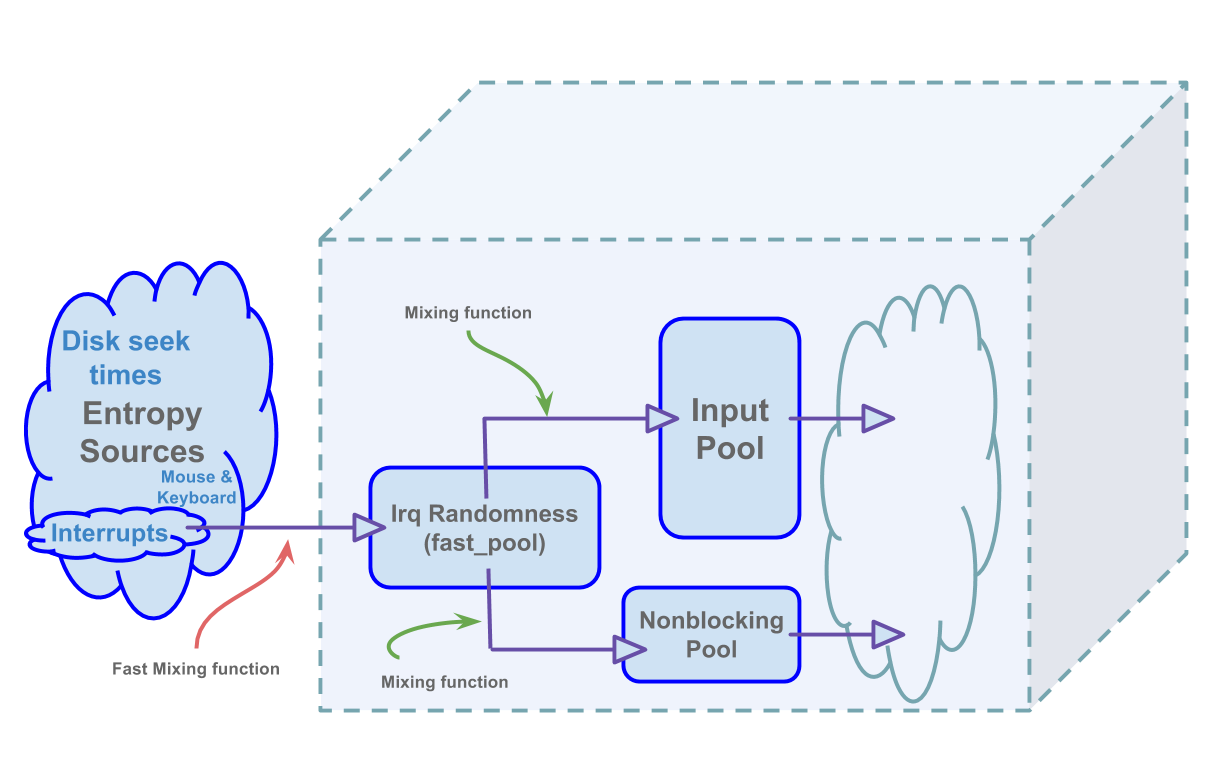
\includegraphics[width=120mm]{img/fast_pool.png}} 
   
   Se l'ultimo interrupt visto dalla
   CPU è troppo recente rispetto all'\emph{interrupt request} attuale, la
   routine \verb+add_interrupt_randomness+ ritorna, sortendo come unico effetto
   un aggiornamento di \verb+irq_randomness+.
   \item Vengono mischiati tutti i bytes della mini-pool di
   \verb+irq_randomness+ presso l'\emph{input pool} (oppure
   presso \emph{nonblocking pool} nel caso questa debba ancora essere
   inizializzata).
   \item Viene accreditata una stima di entropia pari a 1 bit presso la
   \emph{entropy pool} selezionata al passo 3. Tale accreditamento viene omesso
   nel caso in cui non vi sia un contatore di cicli valido per l'architettura
   specifica oppure se si osservano timer interrupt consecutivi (l'accredito è
   analizzato più nel dettaglio in \ref{stimaInput}).
 \end{enumerate} 

 
 \paragraph{} \verb+add_disk_randomness()+ sfrutta la variabilità del 
 \emph{seek time} dei settori dei dischi. Dischi a stato solido sono ovviamente
 quasi completamente inefficaci nell'aggiungere entropia, accedendo ai blocchi di 
 dati in tempo approssimativamente costante. \newline{}Opera sulla struttura 
 \verb+gendisk *disk+ (definita in \verb+include/linux/genhd.c+) specifica per
 il disco che ha generato l'evento.
 In particolare fa uso della struttura \verb+timer_rand_state+ in
 \verb+disk->random+ per l'aggiunta e la stima dell'entropia.
 
 \subsection{La Stima dell'Entropia}\label{stima}
La stima dell'entropia nel LRNG ha come obiettivo di quantificare
l'impredicibilità su cui si può fare affidamento al momento della generazione
di bytes ed è pertanto un'attività di centrale importanza per il LRNG. \\
Si basa su due assunzioni: 
\begin{itemize}
  \item ogni \emph{entropy input} aggiunge una quantità finita di entropia al
  generatore;
  \item ogni output prodotto consuma una quota dell'entropia totale presente
  presso il generatore.
\end{itemize}  
\paragraph{} Sappiamo già (da \ref{interfacceoutput} e \ref{pool} ) che sebbene
il conteggio dell'entropia accumulata nelle pool (mantenuto negli
\emph{entropy counter} di ciascuna) entri in gioco per la produzione di
qualsiasi output, nel caso degli output prodotti dalla \emph{input} e
\emph{blocking pool} è la condizione in base alla quale il LRNG sceglie se
generare o meno bytes verso le interfacce che ne fanno richiesta. \newline Gli
output prodotti in assenza di entropia (provenienti dalla \emph{nonblocking
pool} quando il suo \emph{entropy counter} ha valore zero) sono equivalenti
a quelli prodotti da un generatore di numeri pseudocasuali semplice (ovvero
privo di \emph{entropy inputs}).
Il grado di confidenza che si può avere con l'indipendenza (pur sempre
apparente) di simili output tra loro, seppure elevata, è ovviamente inferiore
rispetto agli output prodotti a partire dall'entropia esterna.
L'utilizzo di sorgenti esterne infatti aumenta, per un attaccante
che abbia accesso a un insieme di output, la difficoltà di inferire informazione
riguardo agli altri valori (passati e futuri) prodotti.
\paragraph{} La stima dell'entropia si basa su due meccanismi, rispettivamente:
\begin{enumerate}
  \item per la stima dei bit di entropia per \emph{entropy input};
  \item per l'accredito presso gli \emph{entropy counter} dei bit di entropia 
  derivati dagli \emph{entropy input}.
\end{enumerate}
Prendendo spunto da \cite{lach} (sez. 2.3.2), ci riferiremo col termine di
\textbf{\emph{entropy estimator}} al complesso di entrambi i meccanismi.

\paragraph{Nota sulla sicurezza:} Il grado di confidenza che un utente può
accordare al LRNG deve tenere conto anche di eventuali vulnerabilità del LRNG
che potrebbero annullare i benefici introdotti dall'aggiunta di entropia
esterna: riportiamo un esempio interessante in questo senso nella sezione
\ref{rdrand} riguardante le vulnerabilità di \emph{RdRand}.

\subsubsection{Assunzioni e vincoli per l'\emph{entropy
estimator}}\label{vincoliStima} 
Prima di analizzare com'è implementato
l'\emph{entropy estimator}, diamo ragione brevemente delle assunzioni e dei
vincoli sugli \emph{entropy input}, individuati nell'articolo di Lacharme
\cite{lach}, a partire dai quali ha preso forma l'implementazione attuale.
\paragraph{Assunzioni:}
\begin{itemize}
  \item le distribuzioni di probabilità sono sconosciute e non uniformi: esse
  infatti cambiano, anche radicalmente, in funzione del contesto in cui si fa
  uso del LRNG, rendendo impossibile (o molto difficile) fare previsioni sugli
  input;
  \item la correlazione fra input è sconosciuta: sebbene sia scontato che vi
  siano delle correlazioni fra input consecutivi (soprattutto se provenienti
  dalla stessa sorgente di entropia), è difficile catturarne la natura;
  \item lo spazio dei campioni è ampio: le differenze tra i \emph{jiffies} sono
  valori a 32 o 64 bit (a seconda dell'architettura) indefinitamente grandi, che
  possono pertanto variare fra $2^{32}$ o $2^{64}$ possibilità;
  \item non è possibile stabilire a priori quale sia la conoscenza di un
  attaccante.
\end{itemize}
\paragraph{Vincoli:}
\begin{itemize}
  \item il tempo per effettuare la stima è limitato: la stima avviene anche al
  termine della gestione dell'interrupt, per cui deve richiedere un tempo di
  esecuzione minimo;
  \item la stima deve essere effettuata a runtime: l'impredicibilità deve essere
  calcolata per ogni input, per cui non è possibile differire la stima
  dell'entropia successivamente all'arrivo di un set di input.
\end{itemize}
 
 \subsubsection{La stima dell'entropia per \emph{entropy
 input}}\label{stimaInput} 
 A seconda delle sorgenti di entropia cambia il modo
 di stimare l'impredicibilità introdotta dallo specifico \emph{entropy input}.
 In ciascuna delle interfacce descritte in \ref{interfacceinput} è implementato
 il meccanismo particolare per l'input in gestione. Specifichiamo che il tempo 
 osservato dal meccanismo di stima dell'entropia
 è sempre misurato solo in \emph{jiffies}, affiché la stima sia sempre
 pessimistica:
 la stima non tiene conto del numero di \emph{cycles} anche quando questo sia
 disponibile e venga utilizzato dalla funzione di mixing.
 
 \paragraph{}\verb+add_device_randomness()+ non implementa alcuna stima di
 entropia, in quanto i valori che vengono presi in input sono quelli che servono
 a distinguere quanto più possibile la configurazione dell'architettura
 presente da tutte le altre. A fronte di avvìi distinti della macchina, il
 contributo di questa routine nell'aggiornamento dello stato interno del
 generatore è sempre lo stesso, ed è per questa ragione che non vi è alcuna
 ``nuova'' impredicibilità da considerare per la stima dell'entropia.
 
 \paragraph{}\verb+add_interrupt_randomness()+ prova a accreditare presso la
 \emph{entropy pool} opportuna un bit di entropia per ogni interrupt ricevuto, a
 meno che non si siano attivati i meccanismi di filtro dell'input descritti in
 \ref{interfacceinput}. In base alla frequenza degli arrivi degli interrupt e
 all'architettura sono possibili tre casi:
 \begin{enumerate}
   \item viene aggiunto il contenuto informativo dell'input alla \emph{fast
   pool} e alla \emph{pool} corretta, viene accreditata l'entropia presso la
   \emph{pool};
   \item  viene aggiunto il contenuto informativo dell'input alla \emph{fast
   pool} e alla \emph{pool} corretta ma non viene accreditata l'entropia presso
   la \emph{pool}: questo è il caso in cui si stanno verificando interrupt dello
   stesso tipo consecutivamente, oppure non vi è un contatore di \emph{cycles}
   valido per l'architettura corrente;
   \item viene aggiunto il contenuto informativo dell'input alla \emph{fast
   pool} ma non presso alcuna \emph{entropy pool}, né viene accreditata
   l'entropia presso la \emph{pool}: è quanto avviene se l'interrupt si è
   verificato a meno di 100 jiffies dall'ultimo aggiornamento della \emph{fast
   pool} oppure il counter della fast pool è congruo a $2^6$ (sebbene sia un
   valore \verb+short+ e possa assumere valori in $2^{16}$ ).
 \end{enumerate}
 
 \paragraph{}\verb+add_input_randomness()+ e \verb+add_disk_randomness()+
 gestiscono gli input a maggior valore entropico, cioè quelli provenienti
 rispettivamente dagli input utente e dagli accessi a disco. Per entrambe le
 routine la stima viene effettuata attraverso la chiamata ad una terza funzione,
 \verb+add_timer_randomness(),+ che si occupa dell'aggiunta dell'entropia presso
 le pool, effettua una stima dell'entropia basata sui primi tre ordini di delta
 ($\delta$) e prova a accreditare la misura stimata presso l'\emph{entropy
 counter} corretto.\newline{}Ogni ordine di $\delta$ è calcolato nel modo
 seguente:
 \begin{enumerate}
   \item $\delta$ (nel codice sorgente, \verb+delta+) è pari al tempo di
   interarrivo tra gli ultimi due input, ovvero tra quello corrente e il suo
   predecessore;\label{delta1}
   \item $\delta_2$ (\verb+delta2+) è pari a $|\delta-\delta_{old}|$, ovvero al
   modulo della differenza tra il $\delta$ calcolato al punto \ref{delta1} e il
   $\delta_{old}$ calcolato per l'ultimo input giunto dalla stessa sorgente di entropia;
   \item $\delta_3$ (\verb+delta3+) è pari a $|\delta_2-\delta_{2\ old}|$.
 \end{enumerate}
 Una volta calcolati i tre ordini di delta, viene considerato per la stima
 dell'entropia quello col valore minore.\\ Durante la chiamata a
 \verb+add_timer_randomness()+ viene disattivata la \emph{preemption}.
 
 \subsubsection{L'accredito di entropia}\label{credit}
 L'accredito di entropia presso le \emph{pool} avviene tramite le routine
 \verb+credit_entropy_bits()+ e \newline{}\verb+credit_entropy_bits_safe()+.
 Quest'ultima si differenzia dalla prima soltanto per un controllo sulla correttezza del
 numero di bits che si vuole accreditare presso la \emph{pool} specificata e
 viene usata nel caso di reseeding provenienti dallo spazio utente
 (\ref{reseeding}).
 \newline{}Si possono accreditare valori positivi o negativi (in tal caso
 parliamo di debito o consumo di entropia) a seconda che si stia aggiungendo
 entropia proveniente dagli \emph{entropy input} oppure si stia prelevando per
 trasferirla dall'\emph{input pool} verso le \emph{output pool} o per produrre un output. 
 \paragraph{}Vogliamo porre l'accento su come vengano trattati in modo
 completamente differente i due casi di accredito e di debito di bit di
 entropia: mentre il debito è gestito tramite un approccio lineare, venendo
 sottratto dagli \emph{entropy counter} della pool un numero di bit esattamente
 pari al numero di bit che si vogliono addebitare, nel caso dell'accredito
 l'aggiunta di bit di entropia contribuisce ad avvicinare asintoticamente
 l'\emph{entropy counter} al suo valore massimo senza mai raggiungerlo. Oltre a
 ciò, nel caso in cui la quantità di entropia stimata per l'\emph{input pool}
 sia prossima al suo valore massimo, viene fatta ``traboccare'' una parte di
 quest'entropia verso una \emph{pool} di output.
 \paragraph{}Ricordiamo che nel conteggio dell'entropia accumulata presso le
 pool l'unità di misura è l'ottavo di bit ($2^{-3}$ bit). Tale accorgimento
 accresce di molto la risoluzione del meccanismo di accredito asintotico di
 bit di entropia presso le pool, facendo sì che possano essere conteggiate
 le aggiunte di entropia degli \emph{entropy input} anche quando la \emph{pool}
 è quasi ``satura''. Ovviamente, per la produzione di bit in output
 vengono considerati solo valori interi.
 
 \paragraph{}Analizziamo di seguito i passi richiesti dall'operazione di
 accredito di entropia:
 \begin{enumerate}
   \item se il numero di bit di entropia da aggiungere è negativo, tale numero
   viene direttamente sottratto dall'\emph{entropy counter};
   \newline se invece tale numero è positivo, viene calcolata quanta parte dei
   bit di entropia stimati vada sommata all'\emph{entropy counter}: sia
   $entropy$ la quantità di entropia presente nella pool, $pool\_size$ la
   massima quantità di entropia che è possibile accumularvi e $add\_entropy$ i
   frazionali di bit che si vogliono accreditare.
   Per dovere di completezza segnaliamo che $add\_entropy$ non può essere
   maggiore della metà della capacità della pool e, nel caso il numero di bit
   che si vogliono accreditare sia maggiore di tale quantità, la parte
   in eccesso viene scartata.
   \newline La quantità di
   entropia che verrà aggiunta al conteggio in $entropy$ sarà dunque pari a:
   \begin{center}
   $new\_credit\leftarrow(pool\_size -
   entropy)*(1-e^{\frac{-add\_entropy}{pool\_size}})$
   \end{center}
   Volendo evitare l'onerosità di calcolo dell'esponeziale nella formula di
   $new\_credit$ è necessario sostituirlo con una sua stima più economica.
   \newline Consideriamo che se $0\leq x\leq\frac{1}{2}$, allora
   $\frac{(1-e^{-x})}{x}\geq
   \frac{(1-e^{-\frac{1}{2}})}{\frac{1}{2}} = 0.7869386805747332$.
   \newline Quando $add\_entropy\leq\frac{pool\_size}{2}$, possiamo
   quindi approssimare per difetto il termine
   $(1-e^{\frac{-add\_entropy}{pool\_size}})$ con $(\frac{add\_entropy}
   {pool\_size})*0.7869\ldots$, sapendo che
   $(1-e^{\frac{-add\_entropy}{pool\_size}})\geq(\frac{add\_entropy}
   {pool\_size})*0.7869\ldots$ 
   \newline Approssimando ancora $0.7869\ldots$ con $3/4=0.75$ si ottiene la
   stima di $new\_credit$ implementata dalla routine:
   \begin{center}
   $new\_credit\leftarrow(pool\_size -
   entropy)*\frac{add\_entropy}
   {pool\_size}*\frac{3}{4}$.
   \end{center}
   \item viene controllato che l'\emph{entropy counter} sia consistente: 
	\begin {itemize}
	  \item se negativo ne viene corretto il valore a 0;
	  \item se maggiore della capacità della pool $pool\_size$ ne viene corretto
	  il valore a $pool\_size$.
	\end{itemize}
   \item controllo sugli accessi concorrenti: se il valore dell'\emph{entropy
   count} è diverso da quello registrato all'inizio della chiamata alla funzione
   deve essere occorso almeno un accredito di entropia concorrente a quello
   presente e deve essere rieseguita l'intera routine di accredito;
   \item configurazione della pool come inizializzata: nel caso in cui la
   \emph{pool} abbia una stima di entropia superiore a 128 bit e non sia ancora
   stata inizializzata, viene configurata come inizializzata. Nel caso in cui la
   \emph{pool} in esame sia la \emph{nonblocking}, viene invocata una routine
   (\verb+prandom_reseed_late()+) che ne inizializza il buffer interno con dei
   valori di 4 bytes senza segno (ottenuti tramite l'invocazione di
   \verb+get_random_bytes()+, quindi originati dalla stessa \emph{pool
   nonblocking}).
   \item step finali nel caso la \emph{pool} in esame sia la \emph{input pool}: 
       \begin{enumerate}
         \item se il numero di bytes di entropia della \emph{pool} è superiore
         della soglia opportuna (64 bytes), cambia il flag di polling delle
         \emph{file operations} consentite sul device file \verb+random+ per
         segnalare la possibilità di accesso non bloccante ai processi in attesa
         di lettura (per il polling su \verb+random+ rimandiamo alla sezione
         \ref{outputUtente});
         \item se la stima di entropia presso l'\emph{input pool} è maggiore di
         $7/8$ della capacità complessiva della \emph{pool}, schedula
         alternatamente la \emph{nonblocking pool} e la \emph{blocking pool}
         perché vengano trasferiti, dalla \emph{input pool} presso una di esse,
         fino a 8 bytes di entropia. Non viene schedulato nulla se la
         \emph{output pool} selezionata è già satura per almeno il 75\%. Questo
         meccanismo è alla base del bilanciamento dell'entropia interna, come
         vedremo più avanti nella sezione \ref{bilanciamento}.
       \end{enumerate}
   
   \end{enumerate}
 
 
 \subsection{La Mixing Function}\label{mixingfunction}
 La \textbf{mixing function} si occupa di mischiare un dato numero di bytes di
 un buffer in input al buffer interno di una specifica pool. Nel caso del LRNG,
 la mixing function è una "buona funzione hash non crittografica" \cite{lach}.
 In assenza di input, essa è equivalente ad un \emph{registro a scorrimento a
 retroazione lineare} (\emph{linear feedback shift register} o \emph{LFSR})
 definito su un campo finito (o campo di Galois) di $2^{32}$ elementi
 ($GF(2^{32})$), con polinomio di feedback $Q(X)=\alpha^3(P(X)-1)+1$ (con
 $\alpha$ primitiva di $GF(2^{32})$) e basato sui polinomi $P(X)$:
 \begin{center}
 $P(X)=X^{128}+X^{104}+X^{76}+X^{51}+X^{25}+X+1$ per la \emph{input pool};
 $P(X)=X^{32}+X^{26}+X^{19}+X^{14}+X^{7}+X+1$ per le \emph{output pool}.
 \end{center}
 La moltiplicazione per $\alpha^3$ è effettuata attraverso una tabella di lookup
 che nel codice è chiamata \textbf{twist table}.
 
 \paragraph{} Il cuore della \emph{mixing function} è costituito dalla
 definizione dei polinomi nella struttura \verb+poolinfo+ e dall'implementazione
 del LFSR nella routine \verb+_mix_pool_bytes()+. 
 \newline \verb+_mix_pool_bytes()+ per ogni byte del buffer in input, esegue le
 operazioni:
 \begin{enumerate}
   \item viene prelevato il byte corrente assieme ai 3 byte che lo seguono.
   Otteniamo una parola $w$ di 4 bytes che viene ruotata del numero
   \verb+input_rotate+ di posizioni (in bit) specificato dalla pool;
   \item viene inizializzato un cursore $i$ con la posizione del
   predecessore dell'ultima parola modificata della \emph{pool};
   \item viene effettuato il calcolo del polinomio $P(X)-1$ per $X=w$
   come:
   \begin{center}
   $w\leftarrow w \oplus pool[i + tap_j]$
   \end{center}
   dove $i$ è la posizione di una parola di 4 bytes della pool e $tap_j$ è la
   potenza j-esima del polinomio $P(X)$ (di cui non consideriamo la potenza 0
   a causa dell'addendo $-1$ in $P(X)-1$); tale operazione viene applicata 
   $\forall\ tap_j \in \left\{128, 104, 76, 51, 25, 1 \right\}$ nel caso della
   \emph{input pool} ($\forall tap_j \in \left\{32, 26, 19, 14, 7, 1 \right\}$
   nel caso delle \emph{output pool}).
   \item viene aggiornata l'i-esima parola della pool con 
   $\alpha^3\left(P(X)-1\right)-1$:
   \begin{center}
   $pool\left[i\right] \leftarrow  \left(w*2^3\right) \oplus
   twist\_table\left[w\ mod(8)\right]$
   \end{center}
   \item il numero di posizioni della rotazione per la prossima iterazione
   \verb+input_rotate+ viene aumentata di 7 posizioni (o 14 alla prima
   iterazione) e ridotta modulo 32;
   \item vengono salvati nella \emph{pool} la posizione \verb+i+ dell'ultima
   parola aggiornata della \emph{pool} e \verb+input_rotate+.
   \item se tra i parametri è definito il buffer di output \verb+out+ ne vengono
   riempiti i primi 16 elementi con 16 valori consecutivi della pool letti al
   contrario (dalla posizione di scrittura nella pool corrente procedendo in
   senso inverso): tali valori sono quelli a maggior contenuto entropico
   perché sono quelli che sono stati letti meno di recente.
 \end{enumerate}
 \begin{center}
 [IMMAGINE MIXING FUNCTION]
 \end{center}
 
 \paragraph{}I polinomi caratteristici attuali sono costruiti in modo da
 garantire, nel caso non vi siano input di entropia, il massimo periodo per gli output di LRNG.
 Condizione necessaria e sufficiente perché il periodo sia massimo è la
 primitività del polinomio di feedback $Q(X)=\alpha^3(P(X)-1)+1$.
 L'attuale versione del LRNG accoglie le modifiche ai polinomi caratteristici
 $P(X)$ delle pool suggerite nell'articolo di Lachman et al. \cite{lach}
 affinché sia garantita la primitività di $Q(X)$. 
 \newline Per una descrizione più approfondita, rimandiamo il lettore alla
 sezione \ref{mixingfunctionchanges} sulla storia di alcuni cambiamenti del
 codice.
 
 \section{L'Output}
 La produzione degli output necessita di un meccanismo per l'estrazione
 dell'entropia che mantenga intatta la sicurezza del generatore. Per
 garantire il rispetto dei vincoli di sicurezza definiti nella sezione
 \ref{sicurezza} il LRNG fa uso di SHA-1 per ``mascherare'' i bytes dello
 stato interno utilizzati per l'estrazione di entropia rispetto ai bytes in
 output prodotti.
 \paragraph{}In questa sezione analizziamo l'estrazione di entropia in funzione
 delle \emph{pool} coinvolte:
 \begin{enumerate}
   \item dalle \emph{output pool} vengono prodotti bytes in output ogni
 volta che viene invocata una tra le interfacce di output descritte in
 \ref{interfacceoutput} ;
 \item dall'\emph{input pool}, quando è disponibile, viene
 estratta entropia 
 \begin{itemize}
   \item ogni volta che vengono richiesti bytes in output dalle
   \emph{pool} di output e queste non hanno sufficiente entropia;
   \item quando l'\emph{input pool} è satura per più di $\frac{7}{8}$ e almeno
   una delle \emph{pool} secondarie è satura meno del 75\%.
 \end{itemize}
 \end{enumerate}
 In particolare, nel primo caso sono generati bytes di entropia per produrre un
 output verso lo spazio utente o lo spazio kernel (\ref{produzioneoutput}), mentre nel
 secondo viene estratta entropia dalla \emph{input pool} per trasferirla presso
 una delle pool di output(\ref{trasferimentoentropia}).
 
 
 
 \subsection{Estrazione di un buffer dalla \emph{pool}}\label{estrazionebuffer}
 L'estrazione di un buffer, ovviamente, non consiste nell'ottenere
 direttamente una porzione più o meno lunga del buffer interno della
 \emph{pool}, quanto piuttosto un suo hash crittograficamente ``robusto''.
 Come abbiamo già affermato in \ref{aggiuntaentropia}, questo è il passaggio più
 delicato in termini di sicurezza e la sua affidabilità è delegata totalmente
 all'adozione della funzione crittografica SHA-1. 
 \paragraph{} L'estrazione implementata dal LRNG consta sostanzialmente di tre
 passi: dapprima produce un hash (quello che vedremo nel dettaglio essere il
 buffer $w$) a partire dai valori interni della \emph{pool}, prosegue estraendo
 dalla \emph{pool} il buffer di 512 bit con maggiore contenuto entropico
 ($extract$) e termina producendo un nuovo hash (sempre via SHA-1) da copiare
 nel buffer di output.
 \paragraph{} Volendo osservare più dettagliatamente la funzione di estrazione
 dell'entropia, implementata dalla routine
 \verb+extract_buf()+, troviamo la procedura seguente:
 \begin{enumerate}
   \item inzializza un buffer $w$ di 5 parole a 32 bit;
   \item applica, per un numero di volte dipendente dalla \emph{pool} (2 per le
   \emph{output pool} e 8 per l'\emph{input pool})  l'hash di SHA-1 ai 512 bit
   della pool che iniziano con la parola in posizione $i$, utilizzando $w$ come
   digest:
   \begin{center}
   $pool\left[i\right]_{512}\leftarrow f_{SHA-1}(w, pool\left[i\right]_{512})$
   \end{center}
   dove $i$ è un cursore inizializzato a zero e incrementato con passo 16 e
   $pool\left[i\right]_{512}$ è il buffer dei 512 bit della \emph{pool}
   dall'inizio della parola in posizione $i$. Da notare che ad ogni iterazione
   vengono anche modificati i valori del digest $w$; 
   \item se l'architettura è \verb+x86+ o \verb+powerPc+, calcola un buffer
   \verb+l+ composto da 5 o 4 \verb+unsigned long+ (rispettivamente nel caso di
   architetture a 32 e 64 bit) tramite la chiamata a
   \verb+arch_get_random_long()+:
   \begin{enumerate}
     \item in \verb+x86+, ogni valore è ottenuto da un'invocazione
     dell'istruzione \verb+RdRand+ delle architetture \emph{Intel onchip}, che
     ritorna un numero casuale dal generatore hardware della
     CPU;\label{rdrandPoint}
     \item in \verb+powerPc+ il buffer è riempito da valori diversi da zero 
     solo se la linea dell'architettura è la \verb+pSeries+: è il
     caso di server basati sulla virtualizzazione hardware, i valori sono
     ottenuti attraverso una chiamata all'interfaccia \verb+H_RANDOM+
     dell'\emph{hypervisor} (se ne espone una).
   \end{enumerate} 
   \item chiama la \emph{mixing function} per il mixing di $w$ nella
   \emph{pool} estraendo da essa il buffer \verb+extract+ di 512 bit, composto
   dai valori della \emph{pool} che sono stati aggiornati meno di recente dalla
   routine per il mixing \verb+mix_pool_bytes()+;
   \item applica uno SHA-1 al buffer estratto usando ancora come digest $w$:
   quest'operazione è fondamentale per crittografare \verb+extract+ e mascherare i
   bit prelevati direttamente dalla pool;
   \item azzera il contenuto del buffer \verb+extract+ (per ragioni di sicurezza,
   contenendo bit copiati direttamente dalla \emph{pool});
   \item mischia i valori di $w$ e li salva nel buffer di output \verb+out+;
   \item azzera il buffer contenente $w$.
 \end{enumerate}
 
 \paragraph{Nota:}Vogliamo evidenziare qui come il punto \ref{rdrandPoint} sia
 in contraddizione con quano affermato dal commento al codice, in cui si afferma
 di non fare alcun uso dei generatori hardware al momento dell'estrazione del
 buffer dalle \emph{pool}. Esamineremo questo fatto nel paragrafo \ref{rdrand}
 su \verb+RdRand+ assieme alle critiche di cui è oggetto.
 
 \subsection{Il trasferimento di entropia}\label{trasferimentoentropia}
 Il LRNG implementa alcuni meccanismi atti a bilanciare la quantità di
 entropia presente al suo interno e garantire che non venga
 sprecata. Perché ciò possa accedere è necessario poter trasferire entropia tra
 le \emph{pool}.
  
 \paragraph{}Per impedire che l'\emph{input pool} sia
 ``prosciugata'' inutilmente, le \emph{output pool} rimangono prive di entropia
 fino al momento in cui viene loro richiesto di produrre un output: solo allora
 vengono trasferiti bytes di entropia verso la
 \emph{pool} che ne ha bisogno.
 Oppure può succedere, al contrario, che il sistema debba accumulare tanta
 entropia da tendere a saturare l'\emph{input pool}: poiché abbiamo visto come
 il meccanismo di accredito di entropia (descritto in \ref{credit} ) incrementi
 in modo asintotico gli \emph{entropy counter}, è ragionevole pensare che se
 l'\emph{input pool} è sufficientemente ``piena'' sia conveniente ``stipare''
 entropia anche presso le \emph{output pool}.
 
 \paragraph{}In entrambi i casi è necessario trasferire entropia dalla
 \emph{intput pool} ad una \emph{pool} secondaria: questo compito è assolto
 dalla routine \verb+xfer_secondary_pool()+.
 
 
 \subsubsection{Dall'\emph{input pool} alle \emph{output
 pool}}\label{trasf_input_output}
 Vediamo in questo paragrafo come opera \verb+xfer_secondary_pool()+.
 
 \paragraph{Idempotenza verso \emph{nonblocking pool}:}Quando viene invocata,
 \verb+xfer_secondary_pool()+ controlla per prima cosa se è stato richiesto un
 trasferimento di entropia verso la \emph{nonblocking pool}: se questa è già
 stata aggiornata negli ultimi 60 secondi, la funzione ritorna senza operare
 alcun effetto. Questo meccanismo di fatto implementa l'idempotenza verso
 accessi frequenti e consecutivi alle interfacce della \emph{pool} non
 bloccante ed è immediato convincersi della sua necessità: un qualunque processo
 (o più processi concorrenti), sia esso nello spazio
 kernel o nello spazio utente, che faccia richieste di numeri randomici di
 qualità inferiore ad un tasso relativamente sostenuto potrebbe esaurire
 velocemente l'entropia accumulata nel generatore e conseguentemente bloccare i
 processi dello spazio utente che invece necessitano di output altamente
 affidabili. 
 
 \paragraph{Controllo sulla disponibilità di entropia corrente:} Per evitare
 che vengano tolti inutilmente bytes di entropia dalla \emph{input pool}, la
 routine controlla, prima di trasferire effettivamente i bytes tramite
 \verb+_xfer_entropy_pool()+, che nella \emph{pool} corrente vi sia meno
 entropia di quella richiesta. \\Continuiamo la descrizione di
 \verb+xfer_entropy_pool()+ attraverso quella di \verb+_xfer_entropy_pool()+.
 
 \paragraph{\textunderscore{}xfer\textunderscore{}entropy\textunderscore{}pool():}
 Questa è la routine che si occupa effettivamente del trasferimento di bytes di
 entropia dalla \emph{input pool}. Oltre che essere estesa da
 \verb+xfer_entropy_pool()+, viene invocata in modo diretto dalla routine per il
 riequilibrio dell'entropia \verb+push_to_pool+ (che
 vedremo in \ref{bilanciamento}).\\
 La routine prende le mosse dall'inizializzazione delle variabili che
 definiscono l'upper e il lower bound dell'entropia trasferibile, stabilendo che
 debbano essere trasferiti non meno di 8 bytes di entropia (corrispondenti alla
 soglia di attivazione per i processi sospesi nella lettura di
 \verb+/dev/random+) e non più di 128 bytes (pari alla dimensione massima di
 una \emph{pool} di output).\\
 Le operazioni successive sono naturalmente conseguenti: 
 \begin{enumerate}
   \item viene estratto un buffer dalla \emph{input pool} con le caratteristiche
   sopra citate attraverso la chiamata \verb+extract_entropy()+ (descritta più
   avanti in \ref{kerneloutput});
   \item viene effettuato il mixing del buffer così estratto attraverso
   \verb+mix_pool_bytes()+ (già descritta nella sezione
   \ref{mixingfunction} sulla \emph{mixing function});
   \item viene aggiornato l'\emph{entropy counter} via
   \verb+credit_entropy_bits()+ (vista in \ref{credit}).
 \end{enumerate}
 
 \subsubsection{Il bilanciamento dell'entropia} \label{bilanciamento}
 Alla fine della sezione \ref{credit} sull'accredito di entropia abbiamo
 descritto il meccanismo per cui, se l'\emph{input pool} ha un entropia
 superiore ai $7/8$ della sua capacità, viene trasferita parte di quest'entropia
 (8 bytes per volta) alternativamente in una delle due \emph{pool} secondarie se
 questa non è già impegnata per oltre il $75\%$ della propria capacità.
 \paragraph{}La routine che viene schedulata da \verb+credit_entropy_bits()+ per
 bilanciare l'entropia in eccesso è \verb+push_to_pool()+, puntata
 dal campo \verb+push_work+ della struttura \verb+entorpy_store+ che modella le
 \emph{pool} di output. \verb+push_to_pool()+ non fa altro che invocare
 \verb+_xfer_secondary_pool+ per trasferire gli 8 bytes di entropia dalla
 \emph{input pool} alla \emph{outpul pool}.
 
 \subsubsection{L'accounting di entropia}\label{account}
 L'accounting nel LRNG è l'operazione che valuta quanti bytes possono essere
 effettivamente prelevati da una pool a fronte di una richiesta di
 una quantità pari a \verb+nbytes+.
 Il modo in cui viene compiuta questa misura cambia a seconda che la
 \emph{pool} sia bloccante o non bloccante: nel primo caso infatti viene
 restituito il minimo tra i bytes di entropia disponibili per l'estrazione e
 \verb+nbytes+, nel secondo il valore di ritorno è lo stesso \verb+nbytes+.
 In entrambi i casi comunque l'\emph{entropy counter} della pool viene
 aggiornato con il valore corretto. La routine addetta all'operazione di accounting è
 \verb+account()+.
 
 \paragraph{account():} Alla routine viene passato come parametro, oltre
 all'intero \verb+nbytes+, anche i valori \verb+min+, che definisce il minimo valore di
 entropia che deve essere estratto, e \verb+reserved+, che indica la quantità
 minima di bytes di entropia che devono essere lasciati nella \emph{pool} dopo
 l'estrazione. \\
 Diamo un breve descrizione degli step principali compiuti dalla funzione:
 \begin{enumerate}
   \item nel caso in cui la pool sia bloccante, la quantità di bytes estraibile
   viene calcolata come la differenza tra i bytes della \emph{pool} e i bytes
   \verb+reserved+ che devono essere lasciati ``per terra'';
   \item viene calcolato il nuovo valore dell'\emph{entropy counter} della
   \emph{pool} garantendo che venga rispettato il vincolo su \verb+reserved+;
   \item se l'\emph{entopy counter} letto all'inizio della routine è stato
   modificato da un altro thread prima che il thread corrente vi abbia eseguito
   il proprio aggiornamento, occorre fare un nuovo tentativo per operare
   l'accounting e viene eseguito un \emph{goto} al punto 1;
   \item se il numero (intero) di bit  dell'\emph{entropy counter} cade sotto
   la soglia \verb+random_write_wakeup_thresh+ (pari a 28 word) viene
   impostato a 1 lo switch \verb+wakeup_write+: questo ha lo scopo di abilitare 
   la scrittura per i processi che invocano la chiamata di sistema
   \verb+poll+ sui device files \verb+/dev/random+ e \verb+/dev/urandom+;
   \item se \verb+wakeup_write+ è stato impostato manda un segnale di wake up
   alla \emph{wait queue} \verb+random_write_wait+: la conseguenza è
   l'esecuzione della routine \verb+random_poll()+ che aggiorna la \emph{poll
   mask} per i device file \verb+random+ e \verb+urandom+;
   \item ritorna con il numero di bytes che è possibile prelevare.
 \end{enumerate} 
 Da notare che durante tutta la sua esecuzione, la funzione di accounting opera
 avendo disabilitato le \emph{interrupt request} per poi ripristinarne lo stato
 al termine della sua esecuzione, attraverso le chiamate a
 \verb+spin_lock_irqsave()+ e \verb+spin_unlock_irqrestore()+.
 
 
 \subsection{La produzione dell'output}\label{produzioneoutput}
Nella sezione \ref{interfacceoutput} abbiamo distinto le interfacce di output
tra quelle esportate verso lo spazio kernel e verso lo spazio utente (i device
file \verb+/dev/random+ e \verb+/dev/urandom+). Analizziamo
l'output del LRNG mantenendo questa distinzione. Le pool interessate a questo
livello sono le \emph{output pool}.



\subsubsection{Output nello spazio kernel}\label{kerneloutput}
Tutte le routine esportate verso lo spazio kernel (\verb+get_random_bytes()+,
\verb+get_random_bytes_arch()+, \\
\verb+generate_random_uuid()+ e \verb+get_random_int()+) producono output in
modo non bloccante: tutte infatti generano valori a partire dal buffer interno
della \emph{nonblocking pool}, con la sola eccezione di \verb+get_random_int()+
che genera valori meno crittograficamente robusti senza consumare l'ammontare
dell'entropia complessiva del generatore. 

\paragraph{} L'output basato sul buffer interno della \emph{nonblocking
pool} è un hash ottenuto tramite la chiamata alla routine
\verb+extract_entropy()+, che cerca di estrarre dalla \emph{pool} un numero di
bytes pari a quello specificato per parametro nel modo seguente:
\begin{enumerate}
  \item trasferisce dalla \emph{input pool} (possibilmente) il numero di bytes
  richisto e li mischia alla \emph{nonblocking pool};
  \item sottrae (addebita) all'\emph{entropy counter} il numero di bytes passato
  per parametro (routine \verb+account()+);
  \item estrae bytes in output dalla \emph{nonblocking pool}
  attraverso la chiamata a \verb+extract_buf()+ finché i bytes estratti sono
  pari al minimo tra il numero di bytes di entropia disponibile e quello
  richiesto dalla chiamata a funzione;
  \item ritorna il buffer complessivo dei bytes estratti.
\end{enumerate}


 \paragraph{}\verb+get_random_bytes()+ è senza dubbio l'interfaccia più
 utilizzata dal kernel: essa si occupa di produrre come output un hash dei bytes
 del buffer interno della \emph{nonblocking pool} attraverso la chiamata alla routine
 \verb+extract_entropy()+. Essa consente l'estrazione di bytes randomici da
 parte delle componenti del kernel - tipicamente quelle che implementano
 alcuni tra driver, protocolli di rete, routines di crittografia, protocolli di
 sicurezza - in modo non bloccante.
 
 \paragraph{}\verb+get_random_bytes_arch()+ utilizza il generatore hardware di
 numeri pseudocasuali specifico per l'architettura in uso se ve n'è uno. Il
 vantaggio nell'uso di un dispositivo hardware risiede nella maggiore velocità
 di questo rispetto ad una implemetazione in software, ma l'utilizzatore deve
 ritenere trusted il \emph{manifacturer} del device e avere la ragionevole
 confidenza nel fatto che questi non abbia inserito in esso back door. Il
 funzionamento della routine è abbastanza semplice: dapprima cerca di riempire
 il buffer passato per riferimento con tanti \verb+long+ quanti sono richiesti
 dal parametro \verb+nbytes+; nel caso non sia stato possibile per un qualche
 motivo estrarre tutti i bytes richiesti, si esegue l'estrazione nel modo
 canonico dalla \emph{nonblocking pool}, ovvero mediante
 \verb+extract_entropy()+ (proprio come avverrebbe in
 \verb+get_random_bytes()+).
 
 \paragraph{}\verb+generate_random_uuid()+ viene utilizzato dai protocolli e
 dalle procedure che necessitano di un \emph{Universally Unique IDentifier}.
 L'uso di base che ne fa il kenrel è quello relativo all'assegnazione di
 \emph{uuid} alle partizioni del filesystem e per i driver per i
 filesystem \emph{Lustre}, \emph{Btrfs}, \emph{ubifs} e \emph{reiser fs} ma,
 come spiegato nel commento al codice, l'interfaccia è esportata per
 consentirne l'uso anche agli eventuali driver esterni al kernel che ne abbiano
 necessità. Un \emph{uuid} è un identificativo composto da 16 bytes, ottenuto
 estraendo 16 bytes randomici dalla nonblocking pool via
 \verb+extract_entropy()+.
 
 \paragraph{}\verb+get_random_int()+ si discosta dalle routine precedenti in
 quanto non consuma bytes di entropia da alcuna \emph{pool}. Il suo uso è
 infatti previsto per i casi in cui servono bytes generati casualmente ma su di
 essi non vi è alcun requisito di sicurezza né di qualità, ma unicamente di
 velocità di calcolo: un consumo dell'entropia del generatore per la loro
 produzione corrisponderebbe pertanto ad uno spreco. La routine produce un
 intero a 32 bit cercando dapprima di prelevarli da un eventuale generatore
 hardware di numeri casuali; in caso non sia possibile, ritorna un hash
 composto a partire dal pid del processo corrente, dal valore attuale del
 contatore dei \emph{jiffies} e del contatore di cicli se implementato.
 
  
\subsubsection{Output nello spazio utente}\label{outputUtente}
 
 Sappiamo che le interfacce per gli output (ma anche gli input) del LRNG nello
 spazio utente sono i due device files \verb+/dev/random+ e \verb+/dev/urandom+:
 questi vengono creati assieme agli altri device files dalla componente in
 \verb+/drivers/char/mem.c+ e hanno i permessi in lettura e scrittura (0666 in
 notazione ottale), mentre le operazioni consentite su di essi sono definite
 nelle struct \verb+file_operations+ rispettivamente \verb+random_fops+ e
 \verb+urandom_fops+. Le \emph{file operations} definite su di essi
 differiscono, com'era da aspettarsi, unicamente per le funzioni di lettura,
 ovvero nell'atto di estrazione degli output del LRNG.
 
\paragraph{extract\textunderscore{}entropy\textunderscore{}user()} Prima di
descrivere le funzioni di lettura è necessario introdurre la routine per
l'estrazione dell'entropia dalle \emph{pool} \verb+extract_entropy_user()+,
l'equivalente di \verb+extract_entropy()+ per
le richieste provenienti dallo spazio utente. \\
Sostanzialmente il suo comportamento è del tutto analogo a quello di
\verb+extract_entropy()+ (che abbiamo descritto in \ref{kerneloutput}):
\begin{enumerate}
  \item trasferisce dalla \emph{pool} primaria (possibilmente) nbytes e li
  mischia alla \emph{pool} secondaria;
  \item preleva e ritorna un hash estratto dalla \emph{pool} passata per
  riferimento.
\end{enumerate}
ma si distingue da essa per alcuni dettagli funzionali e implementativi:
 \begin{itemize}
   \item non viene mai chiamata sulla \emph{input pool} ma
   esclusivamente sulle \emph{pool} di output;
   \item finché ci sono bytes da estrarre, prima dell'estrazione controlla che
   il processo corrente non sia bloccato e, nel caso, chiede al kernel di
   rischedularlo;
   \item copia il buffer dei bytes letti nel buffer in output dello spazio
   utente.
 \end{itemize} 
 
 \paragraph{Lettura da /dev/random:} La funzione addetta
 all'operazione di lettura su \verb+/dev/random+ è \verb+random_read()+, estrae
 dalla \emph{blocking pool} 512 byte di entropia per volta e li consegna al
 buffer nello spazio utente tramite \verb+extract_entropy_user()+ fino a
 raggiungere il numero di bytes \verb+nbytes+ richiesto. Nel caso l'estrazione
 fallisca, l'intera funzione ritorna il codice di errore corrispondente.
 Se non è stato possibile estrarre alcun byte e il file passato per
 riferimento alla routine ha impostato il flag \verb+O_NONBLOCK+, la funzione
 ritorna con vil valore \verb+EAGAIN+, ovvero è consentito il polling del
 processo in lettura. Se invece non è stato possibile prelevare byte entropici e
 la lettura del file è bloccante, la lettura del device file è bloccata in
 attesa che venga segnalato il nuovo superamento della soglia di wakeup da parte
 della \emph{input pool}. Non appena il processo è stato risvegliato, ovvero non
 appena è stata aggiunta sufficiente entropia alla \emph{input pool} da
 superare la soglia di wakeup, invia il codice di errore \verb+ERESTARTSYS+ che
 serve al processo chiamante per re-invocare la chiamata di sistema per la
 lettura del device file. Al termine dell'esecuzione della routine, la funzione
 ritorna con il numero di bytes estratti oppure con l'eventuale codice di errore
 nel caso non sia stato possibile estrarne alcuno.
 
 
 
 \paragraph{Lettura da /dev/urandom:} La lettura degli output dal device file
 \verb+/dev/urandom+ è definita dalla routine \verb+urandom_read()+, che si
 limita a eseguire \verb+extract_entropy_user()+ sulla \emph{nonblocking pool}
 per estrarre i bytes richiesti in output e consegnarli direttamente allo spazio
 utente. 
 
 \paragraph{Blocco dell'output o output continuo:} Pur avendo visto le
 funzioni di lettura non abbiamo ancora chiarito come facciano le due interfacce
 \verb+random+ e \verb+urandom+ rispettivamente a bloccare la produzione dei
 bytes in output oppure a produrli anche in assenza di entropia. La differenza
 funzionale dei due device file tra bloccante e non bloccante risiede non solo
 nelle diverse implementazioni delle funzioni di lettura \verb+random_read()+ e
 \verb+urandom_read()+, ma anche da come cambia il comportamento delle routine
 \verb+extract_entropy_user()+ e \verb+account()+ in funzione delle \emph{pool}
 su cui vengono chiamate.
 
  \paragraph{} In \verb+random_read() extract_entropy_user()+ viene chiamata sulla
 \emph{blocking pool}, prova a trasferire nel buffer dello spazio utente il
 numero di bytes richiesto e produce un valore di ritorno n che può essere:
 \begin{enumerate}
   \item il numero di bytes effettivamente trasferiti se $> 0$:
   \verb+random_read()+ prova a trasferire un altro chunk di massimo 512
   bytes, iterando fino al completamento della richiesta;
   \item 0 se non c'è entropia nelle \emph{pool}: in questo caso il
   comportamento di \verb+/dev/random+ dipende da come è stato impostato
   il flag \verb+O_NONBLOCK+ che, nel caso di \verb+random+, è
   \emph{device specific}(\cite{kerr}):
   \begin{enumerate}
     \item se attivo, una \verb+random_read()+ ritorna immediatamente con un
     errore \verb+EAGAIN+: l'invocazione di una nuova \verb+read()+ sarà quindi
     gestita interamente nello spazio utente;
     \item se disattivato, il processo chiamante è sospeso per essere
     poi ``risvegliato'' al sopraggiungere di nuova entropia in quantità
     sufficiente: una volta sbloccato il processo questo riceve come valore di
     ritorno dalla \verb+read+ il codice di errore ERESTARTSYS, che segnala di
     rieseguire la chiamata di sistema su cui si era bloccato precedentemente.
   \end{enumerate}
   \item un codice di errore ($< 0$) nel caso il flusso di esecuzione
   dell'estrazione si sia interrotto per altri motivi.
 \end{enumerate}
 
 \paragraph{} Quando \verb+extract_entropy_user()+ viene chiamata sulla
 \emph{nonblocking pool} in \verb+urandom_read()+, si comporta in modo diverso:
 in questo caso infatti essa copia nel buffer dello spazio utente esattamente
 il numero di bytes randomici richiesti a prescindere da quanti bytes sono
 conteggiati negli \emph{entropy count} dell'\emph{input pool} e della 
 \emph{nonblocking pool}. Questo è possibile perché la routine
 \verb+account()+ (\ref{account}), su cui si basa \verb+extract_entropy_user()+,
 oltre ad aggiornare l'\emph{entropy counter} distingue a sua volta tra
 \emph{pool} bloccanti e non bloccante ritornando, nel primo caso, con il numero
 di bytes di entropia estraibili e, nel secondo, con il numero stesso di
 bytes richiesti. In questo modo \verb+extract_entropy_user()+, chiamata sulla
 \emph{nonblocking pool}, preleva da essa un hash esattamente della dimensione
 desiderata ignorando la quantità di entropia che contiene.
 
  

 \section{Sicurezza nel LRNG}\label{sicurezza}
 In questa sezione diamo una rapida panoramica di come sono implementati
 i requisiti di sicurezza nel LRNG, mentre per il lettore alla ricerca di una
 descrizione approfondita rimandiamo agli articoli \cite{lach} (sezione 4) e
 \cite{gutt} (sezioni 3.1, 3.4).
 
 \subsection{I requisiti di sicurezza}\label{requisitiSicurezza}
 In \emph{``The Linux Pseudorandom Number Generator Revisited''}
 \cite{lach} (estendendo quanto analizzato in \emph{``Analysis of the Linux
 Random Number Generator''} \cite{gutt}) vengono elencati i seguenti requisiti
 di sicurezza:
 \begin{enumerate}
   \item \textbf{buona stima di entropia:} l'entropia introdotta deve essere
   stimata in modo da rendere difficile per un attaccante prevedere gli output senza
   conoscere gli input;
   \item \textbf{pseudorandomicità:} non deve essere possibile, per un
   attaccante con una conoscenza parziale o totale delle sorgenti di entropia,
   predire i futuri output o conoscere lo stato interno a partire dalla
   conoscenza di output correnti;
   \item \textbf{forward security:} un attaccante che conosca lo stato interno
   del generatore non deve poter ricostruire i vecchi output prodotti
   (\emph{backtracking resistence}), ovvero non deve essere in grado di
   ricostruire i vecchi stati assunti dallo stato interno anche in assenza di
   nuova entropia;
   \item \textbf{backward security:} (detto anche \emph{break in recovery}) un
   attaccante che conosca lo stato interno del generatore ad un dato istante
   non deve poter prevedere gli output futuri del generatore se è stata
   introdotta una quantità sufficiente di entropia dall'esterno.
 \end{enumerate}
 Come viene fatto notare in \cite{lach} i requisiti 3 e 4 assumono che un
 attaccante conosca lo stato interno del generatore ad un dato istante, e
 prevedono che il sistema sia resiliente ad attacchi di tipo crottoanalitico;
 allo stesso tempo, gli autori osservano come sia difficile conoscere in
 pratica lo stato interno del generatore in quanto questo vive ed opera
 interamente all'interno del kernel e non vi sono interfacce che ne consentano
 la lettura in maniera diretta.
 
 
 \paragraph{}Nel seguito di questa sezione tratteremo i requisiti 2, 3 e 4 con
 riferimento alle caratteristiche del LRNG esposte fino a questo momento,
 mentre tralasciamo il requisito 1 in quanto necessiterebbe di
 un'attenzione più teorica rispetto allo scopo del nostro lavoro.
 
 \subsection{Pseudorandomicità}
 Il requisito sulla pseudorandomicità considera il caso in cui l'attaccante
 conosca completamente o in parte le \emph{entropy sources}; di seguito
 esaminiamo il suo soddisfacimento considerando il caso ancora peggiore della
 totale assenza di afflusso di entropia esterna.\\
 Il LRNG applica un feedback al proprio stato interno ogni volta che viene
 estratto un output attraverso la \emph{mixing function} descritta in
 \ref{mixingfunction} . Lacharme \emph{et al.} affermano che non vi sia
 conoscenza di attacchi realizzabili, su un generatore di numeri pseudorandomici
 (PRNG) siffatto, che possa fare a meno della conoscenza dello stato interno:
 questo vale in ragione del fatto che SHA-1 è una funzione crittografica a senso
 unico (o, come troviamo in letteratura, \emph{one-way}) e che dunque è teoricamente
 impossibile derivare informazione sullo stato interno
 a partire dagli output prodotti. L'operazione di \emph{folding} dei bytes
 estratti dalla \emph{pool} rispetto a quelli restituiti come output impedisce
 inoltre di risalire allo stesso hash prodotto da SHA-1.
 
 \subsection{Resilienza alla crittoanalisi}
 Come abbiamo anticipato, i requisiti di sicurezza 3 e 4 (visti in
 \ref{requisitiSicurezza}) assumono che l'attaccante abbia una conoscenza
 parziale o totale dello stato interno del generatore. Prima di vedere come
 il LRNG implementi il \emph{forward} e \emph{backward recovery}, vogliamo
 analizzare velocemente in cosa consista tale conoscenza e quali siano gli
 scenari in cui si possa considerare una possibilità concreta.
 
 \paragraph{} Come già sappiamo (\ref{poolACosaServono}), lo stato interno è
 implementato dalle tre \emph{pool input}, \emph{blocking} e \emph{nonblocking}:
 ne consegue che quando parliamo di conoscenza dello stato interno ci riferiamo
 alla capacità di un osservatore esterno di conoscere i valori nei buffer di
 almeno una di esse. Abbiamo anche osservato in \ref{pool} come SHA-1 sia una
 protezione robusta affinché gli output non ``tradiscano'' nulla sul
 contenuto informativo delle \emph{pool}. Per poter avere accesso ai buffer
 interni alle \emph{pool} è necessario pertanto che l'osservatore sia in una
 condizione (e posizione) particolarmente privilegiata (pensiamo ad esempio al
 caso di \emph{ring deprivileging} e \emph{ring compression} che si può avere
 nella virtualizzazione di un sistema operativo). 
 
 \paragraph{} Per poter fare previsioni sugli output è necessario conoscere lo
 stato delle \emph{pool} di output \emph{blocking} e \emph{nonblocking}.
 Sappiamo però che queste sono tendenzialmente prive di entropia fino al
 momento in cui viene richiesto loro di produrre un buffer in output, ed anche
 in questo caso i bytes di entropia sono consumati all'istante:
 l'attaccante dovrebbe pertanto catturare lo stato del buffer interno della
 \emph{pool} tra il momento in cui avviene il reseeding con i bytes provenienti
 dall'\emph{input pool} (tramite \verb+xfer_secondary_pool()+
 \ref{trasf_input_output}) e quello in cui viene estratto l'hash e mischiato al
 buffer in output; conoscere lo stato interno prima di questa brevissima
 finestra sarebbe intutile a meno di possedere (e quindi aver catturato) anche
 l'hash estratto dalla \emph{input pool} da \verb+xfer_secondary_pool()+.
 Continuando questa ricerca a ritroso, troviamo che l'unico modo per poter fare
 delle previsioni, in modo quanto più possibile deterministico, sugli output di
 almeno una fra le interfacce disponibili, occorre conoscere sia lo stato della
 rispettiva \emph{output pool} che quello della \emph{input pool}. Anche in
 questo caso un attaccante a conoscenza dello stato prima della generazione
 dell'output potrebbe inferire lo stato successivo solo a meno dei 160 bit
 mischiati nuovamente alle \emph{pool} per il meccanismo di feedback: in
 assenza di ulteriori informazioni un attacco generico avrebbe un overhead di
 $O(2^{160})$ e produrrebbe $2^{80}$ soluzioni (\cite{lach}). \\\\
 Possiamo quindi considerare che l'assunzione sulla conoscenza da parte di un
 attaccante dello stato interno, su cui si basano i due requisiti in esame, sia
 fortemente difficile da realizzare.
 
 \paragraph{Forward security:} Secondo Elaine Barker e John Kelsey ( in 
``\emph{Recommendation for random number generation using deterministic random
bit generators}'' \cite{bark}), se un generatore di numeri pseudocasuali, ogni
volta che produce i propri output, lo fa sia attraverso una funzione
\emph{one-way} sia adottando un meccanismo di feedback per aggiornare il
proprio stato interno, allora si può considerare resistente al
\emph{backtracking}  come richiesto dal requisito sul \emph{forward recovery}.
Il LRNG implementa tale requisito utilizzando la primitiva SHA-1 per produrre
l'hash su cui si basano il buffer restituito per output e i bytes per il
feedback verso la \emph{pool} (sezione \ref{produzioneoutput}).
 
 \paragraph{Backward security:} La \emph{backward security} è garantita soltanto
 se si è effettuato un reseeding opportuno dello stato interno tra due richieste
 di output distinte (\cite{bark}). Il meccanismo che implementa il requisito è
 dato dal mancato trasferimento di bytes di entropia dalla \emph{input pool}
 alle \emph{pool} secondarie se la prima non ha accumulato almeno 64 bit di
 entropia: per questo motivo la resistenza a questo genere di attacchi
 dichiarata per il LRNG è pari a 64 bit (\cite{lach}).
 
 
 
 \section{Cos'è cambiato?}
 Nella realizzazione del presente lavoro ci siamo imbattuti spesso nelle
 ``tracce'' lasciate dalle vecchie implementazioni del codice -- dalle
 transizioni tra soluzioni differenti alle ottimizzazioni di varia natura --,
 come ad esempio le incongruenze tra quanto affermato nei commenti del codice,
 le differenza tra il codice attuale e quanto affermato negli articoli e
 la presenza nel codice alcuni rami morti del flusso di esecuzione (provenienti
 da meccanismi funzionali rimossi da poco tempo).\\
 Questa sezione ha lo scopo di ``raccontare'' alcuni fra i cambiamenti che
 abbiamo rintracciato, o perché funzionalmente di rilievo (come la
 modifica al polinomio caratteristico delle \emph{mixing function}) e le
 criticità (e le critiche) che sono emerse recentemente sull'uso del generatore
 hardware di numeri randomici delle ultime architetture \verb+x86+ della
 \emph{Intel}.
 
 
 \subsection{Mixing Function e Polinomio Caratteristico}
 \label{mixingfunctionchanges}
 L'ottimizzazione più evidente avvenuta negli ultimi due anni
 all'implementazione del LRNG risiede nel polinomio caratteristico della
 \emph{mixing function}: come rimarcato nei commenti stessi del codice, la
 \emph{mixing function} utilizzato fin dall'origine non generava, in assenza
 di entropia esterna, una sequenza di stati interni di periodo massimo.
 Questo fatto è stato notato per la prima volta proprio nell'articolo di
 Lacharme \emph{et al.} \emph{``The linux pseudorandom
number generator revisited''} (\cite{lach} a pagina 7), dove si suggerivano
anche le modifiche che si sarebbero dovute applicare ai polinomi caratteristici
relativi alle \emph{pool} primaria e secondarie per rendere massimo tale periodo
in $GF(32)$.

\paragraph{} I cambiamenti suggeriti sono stati accolti dalle nuove versioni
del kernel, così che oggi il polinomio relativo alla \emph{input pool}:
\begin{center}
$P(X)=X^{128}+X^{\textcolor{red}{103}}+X^{76}+X^{51}+X^{25}+X+1$
\end{center}
è diventato:
\begin{center}
$P(X)=X^{128}+X^{\textcolor{blue}{104}}+X^{76}+X^{51}+X^{25}+X+1$
\end{center}
mentre il polinomio caratteristico per le \emph{pool} di output è mutato da:
\begin{center}
$P(X)=X^{32}+X^{26}+X^{\textcolor{red}{19}}+X^{14}+X^{7}+X+1$
\end{center}
a:
\begin{center}
$P(X)=X^{32}+X^{26}+X^{\textcolor{blue}{20}}+X^{14}+X^{7}+X+1$
\end{center}
\paragraph{}I periodi sono così aumentati da meno di $2^{92*32}-1$ a
$2^{128*32}-1$ per la \emph{input pool} e da meno di $2^{26*32}-1$ a $2^{32*32}-1$ per le
\emph{output pool} (sempre da \cite{lach}).

 \subsection{Rimozione di IRQF\textunderscore{}SAMPLE\textunderscore{}RANDOM}
 \label{IRQFSAMPLERANDOM}
 Fino alla versione 3.6 del kernel, era necessario dichiarare direttamente nei
 driver se gli interrupt specifici per ciascuno di essi dovessero essere
 considerati sorgenti di entropia o meno. In \cite{lach} si descrive come, per
 fare ciò, si doveva impostare per ciascuno di essi il flag
 \verb+IRQF_SAMPLE_RANDOM+. Dal 2009 si è iniziato a soppiantare
 \verb+IRQF_SAMPLE_RANDOM+, nella gestione degli interrupt, con un approccio
 completamente automatizzato, al punto da sostituirlo completamente nel 2012
 come affermato dallo stesso Theodore Ts'o in una mail della \emph{Linux Kernel
 Mailing List} (rintracciabile nell'archivio in \cite{tso}):
 \begin{center}
 \emph{The 
 IRQF\textunderscore{}SAMPLE\textunderscore{}RANDOM flag is finally gone\\ from
 the kernel tree, only three years late. \Smiley{} }
 \end{center}
 
 \paragraph{}Il motivo alla base di questa sostituzione furono gli usi
 sbagliati che venivano fatti del flag nell'implementazione dei driver. Durante
 questi tre anni di transitorio, gli interrupts vennero di fatto ignorati come
 sorgenti di entropia perché si è ritenuto non vi si potesse più fare
 affidamento con un sufficiente grado di confidenza e le uniche sorgenti di
 entropia rimaste erano soltanto gli input utente e i \emph{disk timings}
 (pagina 4 di \cite{lach}). Notiamo (come visto in \ref{entropyInputs}) che
 anche nell'implementazione attuale ogni interrupt concorre al più per solo un
 bit all'aumento dell'entropia del generatore, mentre gli input utente e i
 tempi di accesso a disco sono stimati avere un contenuto di entropia pari a 64
 bit.
 
 \subsection{Dibattito su RdRAND}\label{rdrand}
 Nel settembre 2013, sul \emph{New York Times}, esce un articolo (\cite{perl})
 che titola ``\emph{N.S.A. Able to Foil Basic Safeguards of Privacy on Web}'' e
 in cui si afferma, tra le varie cose, che il governo statunitense, nelle vesti
 dell'agenzia \emph{N.S.A.}, avrebbe fatto pressione verso diversi manifacturer
 di hardware per inserire \emph{back doors} nei propri prodotti dedicati alla
 sicurezza.
 \paragraph{}Con riferimento all'articolo del \emph{NYT}, il ``padre'' del LRNG
 Theodore Ts'o pubblica sul suo profilo \emph{Google Plus} \cite{tso2}:
 \begin{center}
 «\emph{I am so glad I resisted pressure from Intel engineers to \\ 
 let /dev/random rely only on the RDRAND instruction.\\   
 To quote from the article below:\newline\newline
``By this year, the Sigint Enabling Project had found\\ 
ways inside some of the encryption chips that scramble\\
information for businesses and governments, either by \\
working with chipmakers to insert back doors...''\newline\newline
Relying solely on the hardware random number generator \\
which is using an implementation sealed inside a chip\\ 
which is impossible to audit is a BAD idea.}»
 \end{center}
 \paragraph{}Taylor Hornby, un ricercatore e programmatore canadese, due mesi
 più tardi afferma in un tweet (\cite{tayl}) di essere riuscito a modificare
 l'istruzione \verb+RDRAND+ per ``\emph{cancellare l'altra entropia}'', ovvero
 l'entropia raccolta dal LRNG senza l'ausilio del generatore hardware dei
 processori \verb+x86+, pubblicando contestualmente l'immagine del codice
 dell'hacking e del suo effetto su \verb+/dev/urandom+. Oltre a ciò, sempre
 Hornby pubblica un suo commento al codice (\cite{tayl2}) in cui mette in
 rilievo alcune contraddizioni dei commenti originali; fra questi, vogliamo rilevare in
 particolare il commento alla routine \verb+get_random_bytes()+ dove
 si evidenzia la non veridicità dell'affermazione, presente nel codice, sul non
 uso di generatori hardware di numeri randomici: 
 \begin{center}
 «\emph{This function is the exported kernel interface.\\  It returns some
 number of good random numbers,\\ suitable for key generation, seeding
 TCP sequence numbers, etc.\\ \textbf{It does not use the hw random number
 generator, if available;}\\ use get\textunderscore{}random\textunderscore{}bytes\textunderscore{}arch() for
 that.}»
 \end{center}
 \paragraph{}Come abbiamo avuto modo di verificare noi
 stessi nel presente lavoro (nelle sezioni \ref{estrazionebuffer} e 
 \ref{kerneloutput}), nelle architetture \verb+x86+ \emph{Intel onchips} viene
 in effetti fatto uso del generatore hardware presente nei chipset durante
 l'estrazione di un buffer di bytes randomici dalle \emph{pool} (la
 chiamata \verb+RDRAND+ è implementata nelle architetture \emph{Intel} in
 \verb+get_random()+).
 L'incoerenza del commento al codice rispetto all'implementazione effettiva deve
 aver tratto in inganno anche gli autori di \cite{lach}: a pagina 4, infatti,
 affermano che nessun generatore hardware di numeri pseudocasuali è coinvolto
 nella produzione di output del LRNG (``\emph{[\ldots]hardware RNGs \ldots are
 not mixed into the Linux PRNG}'').\\
 Le nostre osservazioni pertanto confortano quanto affermato da Hornby.
 \paragraph{}L'hacking compiuto da Hornby però non sembra essere applicabile per
 le versioni del kernel successive alla 3.12.3 ma, come lui stesso afferma, è
 ragionevole non escludere l'esistenza di altri punti deboli negli output del
 LRNG:
 \begin{center}
 «\emph{It's fixed in 3.13-rc2, in that you can't \\
 control /dev/(u)random output, but you can still \\
 weaken some other properties.}»
 \end{center}
 
 \subsection{E in futuro?}
 Sia Guttermann \emph{et al.} in \cite{gutt} che Lacharme \emph{et al.} in
 \cite{lach} sono concordi nella necessità di una documentazione del codice più
 approfondita sull'implementazione del LRNG. Soprattutto, abbiamo notato
 nel nostro lavoro come addirittura il commento di corredo al codice sorgente, oltre
 che carente di dettagli, sia in alcuni punti obsoleto e non coerente rispetto
 al codice stesso che si propongono di descrivere.
 Il bisogno di una documentazione aggiornata è stata alla base della
 pubblicazione degli articoli sopra citati e, con necessaria e molta modestia,
 di questa nostra analisi, e si giustifica considerando la sensibilità degli
 scenari in cui il LRNG deve impiegato e l'affidabilità che conseguentemente
 gli viene richiesta.
 Le problematiche emerse di recente sulla possibile presenza di \emph{back door}
 nelgli stessi chipset utilizzati dal generatore impone un'analisi più
 approfondita e, a nostro avviso, la necessità di rimuovere l'uso
 di generatori hardware dalle routine per l'estrazione dei buffer dalle
 \emph{pool} del LRNG, ancora ad oggi presente.
 
 
 
 \section*{Conclusioni}
 Nel lavoro che abbiamo presentato sono state esposte le funzionalità del Linux
 Random Number Generator, con particolare attenzione alle interfacce
 \verb+/dev/random+ e \verb+/dev/urandom+ esposte verso lo spazio utente.
 Oltre alla descrizione funzionale, è stata analizzata l'implementazione della
 gestione dell'entropia raccolta dal sistema, sia al momento della sua raccolta
 a partire da \emph{entropy inputs} sia relativamente alla produzione di bytes
 di entropia come output.
 
\bibliographystyle{alpha}   
\bibliography{biblio}   
\end{document}
